\chapter{Análisis Estadístico y Resultados}
\label{cap:resultados}

A partir de los los conceptos estadísticos explicados en \cref{cap:estadistica}
y el modelo descripto en \cref{cap:estrategia}, en este Capítulo se presentan
el análisis estadístico de los datos y los resultados obtenidos.

A partir de la función likelihood general (\cref{eq:model}), se puede definir la función
likelihood para este análisis,

\begin{equation}
  L(\bm{n}|\mu_s, \bm{\mu}_p, \bm{s}, \bm{b}, \bm{\alpha}) = \mathcal{P}_\text{SR} \, \times \, \mathcal{P}_\text{CRQ} \, \times \, \mathcal{P}_\text{CRW} \, \times \, \mathcal{P}_\text{CRT} \, \times \, \mathcal{C}_\text{syst} \nonumber \\
   %% &= \Pois(n|\lambda(\mu_s, \bm{\mu}_p, \btheta)) %%\, \times \, \prod_{i \in \text{CR}}
  %% \Pois(n_i|\lambda_i(\mu_s, \bm{\mu}_p, \btheta)) \times C_\text{syst} (\btheta^0, \btheta) \label{eq:model}
  \label{eq:likelihood}
\end{equation}
%
donde $\bm{n}$ es el número de eventos observado en cada región, y $\mu_s$ es la
intensidad de la señal y es el parámetro de interés del análisis.
demás parámetros son parámetros nuisance. Por un lado los parámetros de
normalización de los fondos ($\bm{\mu}_p$), en este caso $\mu_Q$ para el fondo
de {\gjet}, $\mu_W$ para {\wgam} y $\mu_T$ para {\ttgam}. El número de eventos
esperado de señal y fondo en cada región esta dado por $\bm{s}$ y $\bm{b}$, y
provienen de las muestras MC o de los calculados a partir de los datos como se
describe en \cref{cap:fondos}. Los parámetros $\alpha$ parametrizan las
incertezas sistemáticas (descriptas en el \cref{cap:sistematicos}) en la señal y
el fondo utilizando una distribución Gausiana.

A partir de la funcion likelihood, se construye el estadistico de pueba como el \emph{profile likelihood ratio},

\begin{equation}
  q_{\mu_s} = -2 \ln \left( \frac{L(\mu_s, \doublehat{\btheta})}{L(\hat{\mu_s},\hat{\btheta})} \right)
\end{equation}
%
que será utilizado en este análisis, para poner a prueba la compatibilidad de
los datos observados con las predicciones del SM.

Con el ajuste simultaneo a los datos en las CR (o en las CR y SR), los
parámetros descriptos anteriormente pueden ser estimados teniendo en cuenta
apropiadamente sus correlaciones e incertezas. Además, como los parámetros
de normalización de los fondos ($\bm{\mu}_p$) dependen esencialmente de las
regiones de control donde mayor estadística con una alta estadística (respecto a la SR),
se reduce el impacto de estas incertezas en las SR.


El análisis estadístico se implementó utilizando \textsc{HistFitter}\cite{HistFitter}, una herramienta
desarrollada por el grupo de SUSY de ATLAS, que es básicamente una interfaz de
\textsc{RooFit}, \textsc{RooStats}\cite{Moneta:2010pm} y
\textsc{HistFactory}\cite{Cranmer:1456844}, de forma de facilitar el análisis
estadístico. Además el hecho de utilizar una misma herramienta en distintos
análisis dentro de ATLAS, permite que su combinación estadística sea mas
sencilla.




%% The profile LLR is obtained from a simultaneous fit to the contributions
%% from Standard Model background and supersymmetric signal
%% models in a given signal region and its associated background
%% control regions, which are all by design statistically independent.
%% Cross-contamination of backgrounds across control region
%% boundaries and the propagation of statistical and systematic uncertainties is cleanly taken into account.


% Cuando se realiza el ajuste simultaneo en las CR,
%% When fitting CRs simultaneously, common normalizations are allowed in order to correctly take into
%% account the other background contamination in a given CR. Experimental systematic uncertainties are
%% correlated across the CRs and a SR. Sample-dependent theory systematics are uncorrelated.


%% By the simultaneous fit to the data in CRs or to the data in CRs and in a SR, these free and nuisance
%% parameters above can  be optimized with proper correlations and errors. In addition, by constraining the
%% parameters on background components mainly by the control regions with large statistics, the impacts of
%% these uncertainties in the SRs are reduced.


%% \begin{itemize}
%% \item {\bf Discovery fit:} the SR is added to the fit together with a generic non-SM signal component, which is neglected in the CRs. The background prediction achieved is this
%% way conservative since any signal contribution in the CRs is attributed to background and thus results in a possible overestimation of the background in the SRs. As shown above, however, this contribution is expected to be negligible.
%% \item {\bf Exclusion fit} both CRs and SRs are used in the fit. The signal contribution is taken into account as predicted by the tested SUSY model in all the regions.
%% \end{itemize}



%--------------
% Bkg-only fit
%--------------
\section{Validación del Modelo o Ajuste de solo-fondo o ...} \label{sec:bkgonlyfit}

Para validar  los métodos utilizados para estimar los
fondos, se realiza un ajuste simultáneo utilizando únicamente las CR.
%% A este ajuste se lo denomina de solo-fondo.
El objetivo de este ajuste es estimar el fondo total esperado en las VR y las
SR, sin hacer ninguna suposición del modelo de señal. Solo las muestras de fondo
son utilizadas en el modelo, y las CR se suponen libres de contaminación de
señal. El ajuste solo se realiza en las CR, y los procesos de fondo dominantes
son normalizados al número de eventos observado en cada una de las regiones. La
función likelihood utilizada es la de la \cref{eq:likelihood} sin el término de la
SR. Como los parámetros de la pdf correspondientes al fondo son compartidos
entre las diferentes regiones, luego el resultado del ajuste puede ser utilizado para
predecir el número de eventos en las VR y SR.

Las predicciones a partir del ajuste en las CR son independientes del número de
eventos observado en cada SR y VR, lo que permite una comparación no sesgada entre el número de eventos predicho y
observado en cada región.
Los resultados de este ajuste extrapolados a las SR, también son importantes para que
grupos externos al experimento puedan hacer una prueba de hipótesis en un modelo de nueva
física, no realizado por ninguno de los experimentos. %% Debido a la complejidad de
%% estos ajustes resulta difícil reconstruirlos para las persones ajenas a los
%% experimentos.

En las siguientes secciones se muestran los resultados obtenidos
en las distintas regiones del análisis.



% Control Regions
\subsection{Resultados en las regiones de control}

En la \cref{tab:bkgonly_mus} se presentan los parámetros de normalización de
los fondos {\wgam} ($\mu_W$), {\ttgam} ($\mu_T$) y {\gjet}
($\mu_Q$), obtenidos del ajuste de realizado en las regiones de control correspondientes.
El número de eventos predicho para cada proceso de fondo antes y después del ajuste en
las regiones de control puede verse en \cref{tab:fit_result_crl,tab:fit_result_crh}, al
igual que el número de eventos observado.


\begin{table}[!htbp]
  \centering

  \caption{Factores de normalización para los fondos
    {\wgam} ($\mu_{W}$), {\ttgam} ($\mu_{T}$) y {\gjet} ($\mu_{Q}$), obtenidos
    del ajuste combinado en las CR. Las incertezas mostradas son solo estadísticas.}
  \label{tab:bkgonly_mus}

  \begin{tabularx}{0.8\textwidth}{LCCC} %cccc}
    \hline
    &       $\mu_{Q}$ &       $\mu_{W}$ &       $\mu_{T}$ \\
    \hline
    \SRL & $0.94 \pm 0.44$ & $1.34 \pm 0.89$ & $1.40 \pm 0.77$ \\
    \SRH & $1.22 \pm 0.58$ & $1.24 \pm 0.39$ & $0.54 \pm 0.37$ \\
    \hline
  \end{tabularx}

\end{table}


\begin{table}[!htbp]
  \centering

  \caption{Resultados del ajuste en las CR correspondientes a {\SRL}, con una luminosidad integrada total de 20.3 \ifb.
    El número de eventos observado es comparado con el número de eventos esperado de fondo, después de la correspondiente
    normalización en las CR. En la parte inferior de la tabla se muestran también lo valores nominales del fondo antes de
    la correspondiente normalización. Las incertezas incluyen la incerteza estadística y sistemática.}
  \label{tab:fit_result_crl}

  {\small\begin{tabularx}{\textwidth}{|z{3.2mm}|z{5cm}RRR}
\hline
\multicolumn{2}{l}{\hspace{6.5mm} \bf Regiones de control}           & {\CRQL}            & {\CRWL}            & {\CRTL}              \\
\hline
\multicolumn{2}{l}{\hspace{6.5mm} Eventos observados}                             & $1348$              & $8$              & $18$                    \\
\hline
\multirow{11}{*}{\rotatebox[origin=c]{90}{Después}} & Eventos esperados SM                           & $1347.21 \pm 36.51$          & $8.00 \pm 2.75$          & $18.00 \pm 4.16$              \\
\cline{2-5}
 & {\wgam}                                 & $0.28 \pm 0.27$          & $5.24 \pm 3.07$          & $3.15 \pm 1.94$              \\
 & {\ttgam}                                & $2.22 \pm 1.31$          & $1.33 \pm 0.73$          & $10.66 \pm 4.92$              \\
 & {\ttgam} (had)                          & $28.46 \pm 16.90$          & $0.00 \pm 0.00$          & $0.00 \pm 0.00$              \\
 & {\vqqgam}                               & $39.30 \pm 24.90$          & $0.00 \pm 0.00$          & $0.00 \pm 0.00$              \\
 & {\tgam}                                 & $0.24 \pm 0.04$          & $0.22 \pm 0.06$          & $1.24 \pm 0.24$              \\
 & {\zllgam}                               & $0.08_{-0.08}^{+0.10}$          & $0.14_{-0.14}^{+0.14}$          & $0.11_{-0.11}^{+0.11}$              \\
 & {\znngam}                               & $0.00 \pm 0.00$          & $0.00 \pm 0.00$          & $0.00 \pm 0.00$              \\
 & {\gjet}                                 & $1155.79 \pm 68.55$          & $0.13 \pm 0.04$          & $0.01 \pm 0.01$              \\
 & $e\rightarrow\gamma$                    & $5.34 \pm 0.89$          & $0.26 \pm 0.05$          & $1.29 \pm 0.21$              \\
 & $j\rightarrow\gamma$                    & $115.48 \pm 54.49$          & $0.69 \pm 0.32$          & $1.54 \pm 0.72$              \\
\hline
\multirow{11}{*}{\rotatebox[origin=c]{90}{Antes}} & Eventos esperados SM                            & $1397.30$          & $6.29$          & $14.14$              \\
\cline{2-5}
& {\wgam}                                & $0.21$          & $3.90$          & $2.34$              \\
& {\ttgam}                  & $1.59$          & $0.95$          & $7.61$              \\
& {\ttgam} (had)         & $20.31$          & $0.00$          & $0.00$              \\
& {\vqqgam}                   & $29.25$          & $0.00$          & $0.00$              \\
& {\tgam}                  & $0.24$          & $0.22$          & $1.24$              \\
& {\zllgam}    & $0.08$          & $0.14$          & $0.11$              \\
& {\znngam}      & $0.00$          & $0.00$          & $0.00$              \\
& {\gjet}                                & $1224.79$          & $0.14$          & $0.01$              \\
& $e\rightarrow\gamma$             & $5.34$          & $0.26$          & $1.29$              \\
& $j\rightarrow\gamma$             & $115.48$          & $0.69$          & $1.54$              \\
\hline
\end{tabularx}
}

\end{table}


\begin{table}[!htbp]

  \caption{Resultados del ajuste en las CR correspondientes a {\SRH}, con una luminosidad integrada total de 20.3 \ifb.
    El número de eventos observado es comparado con el número de eventos esperado de fondo, después de la correspondiente
    normalización en las CR. En la parte inferior de la tabla se muestran también lo valores nominales del fondo antes de
    la correspondiente normalización. Las incertezas incluyen la incerteza estadística y sistemática.}
  \label{tab:fit_result_crh}

  \begin{tabularx}{\textwidth}{z{5cm}RRR}
\hline
{\bf Regiones de control}           & {\CRQH}     & {\CRWH}            & {\CRTH}              \\
\hline
Eventos observados          & $216$              & $25$              & $17$                    \\
\hline
Eventos esperados SM        & $216.03 \pm 14.53$          & $25.00 \pm 4.99$          & $17.00 \pm 4.08$              \\
\hline
{\wgam}         & $0.10 \pm 0.08$          & $19.32 \pm 5.62$          & $4.66 \pm 1.43$              \\
{\ttgam}          & $0.04 \pm 0.04$          & $1.91 \pm 1.34$          & $6.88 \pm 4.63$              \\
{\ttgam} (had)          & $0.31 \pm 0.24$          & $0.00 \pm 0.00$          & $0.00 \pm 0.00$              \\
V($\to$ qq)$+\gamma$          & $3.46 \pm 1.53$          & $0.00 \pm 0.00$          & $0.00 \pm 0.00$              \\
single-$t$ + $\gamma$          & $0.01_{-0.01}^{+0.02}$          & $0.54 \pm 0.06$          & $1.51 \pm 0.18$              \\
Z($\rightarrow\ell\ell$) + $\gamma$          & $0.00 \pm 0.00$          & $0.57 \pm 0.57$          & $0.19_{-0.19}^{+0.19}$              \\
Z($\rightarrow\nu\nu$) + $\gamma$          & $0.00 \pm 0.00$          & $0.00 \pm 0.00$          & $0.00 \pm 0.00$              \\
$\gamma$ + jet          & $193.31 \pm 16.91$          & $0.02_{-0.02}^{+0.94}$          & $0.00 \pm 0.00$              \\
$e\rightarrow\gamma$ fakes          & $0.27 \pm 0.04$          & $0.49 \pm 0.08$          & $2.31 \pm 0.37$              \\
$j\rightarrow\gamma$ fakes          & $18.52 \pm 8.70$          & $2.14 \pm 0.99$          & $1.46 \pm 0.68$              \\
\hline
Eventos esperado SM (MC/DD)              & $179.24$          & $22.94$          & $22.04$              \\
\hline
MC {\wgam}               & $0.08$          & $15.62$         & $3.76$              \\
MC {\ttgam}              & $0.08$          & $3.57$          & $12.82$              \\
MC {\ttgam} (had)        & $0.58$          & $0.00$          & $0.00$              \\
MC {\vqqgam}             & $2.80$          & $0.00$          & $0.00$              \\
MC {\tgam}               & $0.01$          & $0.54$          & $1.51$              \\
MC {\zllgam}             & $0.00$          & $0.57$          & $0.19$              \\
MC {\znngam}             & $0.00$          & $0.00$          & $0.00$              \\
MC {\gjet}               & $156.91$        & $0.02$          & $0.00$              \\
DD $e\rightarrow\gamma$  & $0.27$          & $0.49$          & $2.31$              \\
DD $j\rightarrow\gamma$  & $18.50$         & $2.14$          & $1.46$              \\
\hline
\end{tabularx}


\end{table}


\begin{figure}[!htbp]
  \centering

  \includegraphics[width=0.49\textwidth]{can_crql_met_et_afterFit}
  \includegraphics[width=0.49\textwidth]{can_crql_rt4_afterFit} \\

  \includegraphics[width=0.49\textwidth]{can_crwl_met_et_afterFit}
  \includegraphics[width=0.49\textwidth]{can_crwl_rt4_afterFit} \\

  \includegraphics[width=0.49\textwidth]{can_crtl_met_et_afterFit}
  \includegraphics[width=0.49\textwidth]{can_crtl_rt4_afterFit} \\

   \caption{Distribuciones observadas de V1 (izquierda) y V2 (derecha) en las
     regiones de control {\CRQL} (arriba), {\CRWL} (medio) y {\CRTL} (abajo),
     después del ajuste combinado.}
   \label{fig:bkgfit_crl_after}

\end{figure}


\begin{figure}[!htbp]
  \centering

  \includegraphics[width=0.49\textwidth]{can_crqh_met_et_afterFit}
  \includegraphics[width=0.49\textwidth]{can_crqh_rt4_afterFit} \\

  \includegraphics[width=0.49\textwidth]{can_crwh_met_et_afterFit}
  \includegraphics[width=0.49\textwidth]{can_crwh_rt4_afterFit} \\

  \includegraphics[width=0.49\textwidth]{can_crth_met_et_afterFit}
  \includegraphics[width=0.49\textwidth]{can_crth_rt4_afterFit} \\

  \caption{Distribuciones observadas de V1 (izquierda) y V2 (derecha) en las
    regiones de control {\CRQH} (arriba), {\CRWH} (medio) y {\CRTH} (abajo),
    después del ajuste combinado.}
  \label{fig:bkgfit_crh_after}

\end{figure}





%% Validation Regions
\subsection{Resultados en las regiones de validación}

Los factores de normalización calculados a partir del ajuste simultáneo en las CR,
detallados en \cref{tab:bkgonly_mus}, son utilizados para estimar los fondos en las
VR, donde se compara el fondo esperado con los datos observados, para validar
la extrapolación que luego se hará a la SR.

Las distribuciones de algunos observables en estas regiones pueden verse en \cref{fig:bkgfit_vrl,fig:bkgfit_crh}.
El número de eventos de fondo predicho esta en buen acuerdo con el número de eventos
observado dentro de las incertezas, lo que permite validar el método empleado y la viabilidad de
utilizar la depredación del número de eventos de fondo en las SR.

Por lo tanto, se procedió a la utilización de los datos experimentales en las regiones
de señal, cuyos resultados pueden verse en la siguiente sección.



%%ors determined for \wgamma\ ($\mu_{W}$), \ttbargam\ ($\mu_{T}$) and QCD prompt photon production ($\mu_{Q}$) are shown in \Tab \ref{tab:fit_bkgonly_mus}. %The $\mu_{W}$ value is consistent
%% %% %with unity within uncertinties. %As expected, $\mu_{Q}$ is way smaller, since the statistics for the smeared pseudo-data is artificially enhanced.
%% The systematic uncertainties in the two signal regions  after the background fit are summarized in \Fig \ref{fig:fit_unc_nuisance_SR}. No profiling of the systematics uncertainties is observed. %hopefully
%% The correlations of these systematics uncertainties and the normalizations are shown in \Fig \ref{fig:fit_corr_SR}. % What do we observe here?

%% Los resultados del ajuste y el número de eventos en los datos observados se
%% presentan en la \cref{tab:fit_result_vrl,tab:fit_result_vrh} para las distintas
%% regiones de validación.


\begin{table}[!htbp]

  \caption{Resultados del ajuste en las VR correspondientes a {\SRL}.
    El número de eventos observado es comparado con el número de eventos esperado de fondo, después de la correspondiente
    normalización en las CR. Las incertezas incluyen la incerteza estadística y sistemática.}
  \label{tab:fit_result_vrl1}

  \begin{tabularx}{\textwidth}{z{4cm}RRRR}
\hline
{\bf Regiones de validación}                  & VRQ            & VRM75            & VRM100            & VRR              \\
\hline
Eventos observados        & $0$            & $54$              & $7$              & $24$                    \\
\hline
Eventos esperados SM    & $0.39 \pm 0.23$  & $51.17 \pm 47.04$          & $13.24 \pm 5.51$          & $24.32 \pm 6.26$              \\
\hline
{\wgam}          & $0.04 \pm 0.04$    & $0.89 \pm 0.79$          & $0.45 \pm 0.40$          & $6.82 \pm 5.74$              \\
{\ttgam}          & $0.30 \pm 0.20$             & $2.55 \pm 1.65$          & $1.54 \pm 1.01$          & $4.74 \pm 2.80$              \\
{\ttgam}  (had)    & $0.02 \pm 0.02$         & $1.69 \pm 1.08$          & $0.38 \pm 0.25$          & $0.00 \pm 0.00$              \\
{\vqqgam}          & $0.00 \pm 0.00$              & $2.45 \pm 2.17$          & $0.82 \pm 0.82$          & $0.00 \pm 0.00$              \\
{\tgam}          & $0.01 \pm 0.01$             & $0.25 \pm 0.10$          & $0.15 \pm 0.06$          & $0.45 \pm 0.08$              \\
{\zllgam}         & $0.00 \pm 0.00$          & $0.08_{-0.08}^{+0.08}$          & $0.04_{-0.04}^{+0.04}$          & $0.08_{-0.08}^{+0.08}$              \\
{\znngam}         & $0.00 \pm 0.00$           & $0.10_{-0.10}^{+0.12}$          & $0.07_{-0.07}^{+0.07}$          & $1.71_{-1.71}^{+1.75}$              \\
{\gjet}        & $0.01_{-0.01}^{+0.07}$            & $35.97_{-35.97}^{+44.72}$          & $7.87 \pm 4.47$          & $2.37 \pm 1.17$              \\
$e\rightarrow\gamma$           & $0.01 \pm 0.00$        & $2.56 \pm 0.72$          & $1.32 \pm 0.43$          & $6.09 \pm 1.14$              \\
$j\rightarrow\gamma$           & $0.00 \pm 0.00$          & $4.63 \pm 2.41$          & $0.60 \pm 0.33$          & $2.06 \pm 0.98$              \\
\hline
%% Eventos esperados SM (MC/DD)              & $0.29$           & $51.24$          & $12.83$          & $21.36$              \\
%% \hline
%% MC W + $\gamma$          & $0.03$                & $0.66$          & $0.33$          & $5.08$              \\
%% MC $t\bar{t}$ + $\gamma$          & $0.21$         & $1.82$          & $1.10$          & $3.39$              \\
%% MC $t\bar{t}$ + $\gamma$ (had)          & $0.01$            & $1.20$          & $0.27$          & $0.00$              \\
%% MC V($\to$ qq)$+\gamma$          & $0.00$             & $1.82$          & $0.61$          & $0.00$              \\
%% MC single-$t$ + $\gamma$          & $0.01$               & $0.25$          & $0.15$          & $0.45$              \\
%% MC Z($\rightarrow\ell\ell$) + $\gamma$          & $0.00$              & $0.08$          & $0.04$          & $0.08$              \\
%% MC Z($\rightarrow\nu\nu$) + $\gamma$          & $0.00$                & $0.10$          & $0.07$          & $1.71$              \\
%% MC $\gamma$ + jet          & $0.01$              & $38.11$          & $8.34$          & $2.51$              \\
%% DD $e\rightarrow\gamma$         & $0.01$             & $2.56$          & $1.32$          & $6.09$              \\
%% DD $j\rightarrow\gamma$         & $0.00$              & $4.63$          & $0.60$          & $2.06$              \\
%% \hline
\end{tabularx}


\end{table}


\begin{table}[!htbp]

  \caption{Resultados del ajuste en las VR correspondientes a {\SRL}.
    El número de eventos observado es comparado con el número de eventos esperado de fondo, despues de la correspondiente
    normalizacion en las CR. Las incertezas incluyen la incerteza estadistica y sistematica.}
  \label{tab:fit_result_vrl2}

  \begin{tabularx}{\textwidth}{z{4cm}RRRR}
\hline
{\bf Regiones de validación}                   & VRWR            & VRWM            & VRTR            & VRTM              \\
\hline
Eventos observados                             & $0$             & $5$             & $1$             & $3$                    \\
\hline
Eventos esperados SM                           & $0.20 \pm 0.15$          & $3.41 \pm 1.41$          & $0.76 \pm 0.30$          & $3.52 \pm 0.84$              \\
\hline
{\wgam}               & $0.13 \pm 0.10$          & $2.39 \pm 1.47$          & $0.04 \pm 0.03$          & $1.04 \pm 0.65$              \\
{\ttgam}              & $0.04_{-0.04}^{+0.07}$   & $0.41 \pm 0.21$          & $0.46 \pm 0.28$          & $1.86 \pm 0.92$              \\
{\ttgam} (had)        & $0.00 \pm 0.00$          & $0.00 \pm 0.00$          & $0.00 \pm 0.00$          & $0.00 \pm 0.00$              \\
{\vqqgam}             & $0.00 \pm 0.00$          & $0.00 \pm 0.00$          & $0.00 \pm 0.00$          & $0.00 \pm 0.00$              \\
{\tgam}               & $0.03 \pm 0.02$          & $0.04 \pm 0.01$          & $0.08 \pm 0.03$          & $0.19 \pm 0.04$              \\
{\zllgam}             & $0.00 \pm 0.00$          & $0.06_{-0.06}^{+0.06}$   & $0.02_{-0.02}^{+0.02}$   & $0.00 \pm 0.00$              \\
{\znngam}             & $0.00 \pm 0.00$          & $0.00 \pm 0.00$          & $0.00 \pm 0.00$          & $0.00 \pm 0.00$              \\
{\gjet}               & $0.00 \pm 0.00$          & $0.00 \pm 0.00$          & $0.00 \pm 0.00$          & $0.00 \pm 0.00$              \\
$e\rightarrow\gamma$  & $0.00 \pm 0.00$          & $0.07 \pm 0.02$          & $0.08 \pm 0.02$          & $0.17 \pm 0.03$              \\
$j\rightarrow\gamma$  & $0.00 \pm 0.00$          & $0.43 \pm 0.21$          & $0.09 \pm 0.04$          & $0.26 \pm 0.12$              \\
\hline
%% MC exp. SM events              & $0.16$          & $2.68$          & $0.62$          & $2.72$              \\
%% \noalign{\smallskip}\hline\noalign{\smallskip}
%%         MC exp. W + $\gamma$ events         & $0.09$          & $1.78$          & $0.03$          & $0.77$              \\
%%         MC exp. $t\bar{t}$ + $\gamma$ events         & $0.03$          & $0.29$          & $0.33$          & $1.33$              \\
%%         MC exp. $t\bar{t}$ + $\gamma$ (had) events         & $0.00$          & $0.00$          & $0.00$          & $0.00$              \\
%%         MC exp. V($\to$ qq)$+\gamma$ events         & $0.00$          & $0.00$          & $0.00$          & $0.00$              \\
%%         MC exp. single-$t$ + $\gamma$ events         & $0.03$          & $0.04$          & $0.08$          & $0.19$              \\
%%         MC exp. Z($\rightarrow\ell\ell$) + $\gamma$ events         & $0.00$          & $0.06$          & $0.02$          & $0.00$              \\
%%         MC exp. Z($\rightarrow\nu\nu$) + $\gamma$ events         & $0.00$          & $0.00$          & $0.00$          & $0.00$              \\
%%         MC exp. $\gamma$ + jet events         & $0.00$          & $0.00$          & $0.00$          & $0.00$              \\
%%         DD exp. $e\rightarrow\gamma$ fakes events         & $0.00$          & $0.07$          & $0.08$          & $0.17$              \\
%%         DD exp. $j\rightarrow\gamma$ fakes events         & $0.00$          & $0.43$          & $0.09$          & $0.26$              \\

%% \noalign{\smallskip}\hline\noalign{\smallskip}
\end{tabularx}


\end{table}


\begin{table}[!htbp]

  \caption{Resultados del ajuste en las VR correspondientes a {\SRH}.
    El número de eventos observado es comparado con el número de eventos esperado de fondo, después de la correspondiente
    normalización en las CR. Las incertezas incluyen la incerteza estadística y sistemática.}
  \label{tab:fit_result_vrh1}

  \begin{tabularx}{\textwidth}{LRR}
\hline
{\bf Regiones de validación}           & VRQ                      & VRH                          \\
\hline
Eventos observados                     & $2$                      & $4$                          \\
\hline
Eventos esperados SM                   & $0.89 \pm 0.32$          & $3.39 \pm 1.69$              \\
\hline
{\wgam}                                & $0.34 \pm 0.19$          & $1.18 \pm 0.55$              \\
{\ttgam}                               & $0.07 \pm 0.05$          & $0.11 \pm 0.08$              \\
{\ttgam} (had)                         & $0.01 \pm 0.01$          & $0.00 \pm 0.00$              \\
%% {\vqqgam}                              & $0.00 \pm 0.00$          & $0.00 \pm 0.00$              \\
{\tgam}                                & $0.03 \pm 0.01$          & $0.01 \pm 0.00$              \\
{\zllgam}                              & $0.02_{-0.02}^{+0.02}$   & $0.00 \pm 0.00$              \\
{\znngam}                              & $0.08_{-0.08}^{+0.08}$   & $1.60_{-1.60}^{+1.61}$       \\
{\gjet}                                & $0.19 \pm 0.11$          & $0.00 \pm 0.00$              \\
$e\rightarrow\gamma$                   & $0.00 \pm 0.00$          & $0.15 \pm 0.03$              \\
$j\rightarrow\gamma$                   & $0.17 \pm 0.09$          & $0.34 \pm 0.16$              \\
\hline
%% MC exp. SM               & $0.86$          & $3.25$              \\
%% \hline
%% MC W + $\gamma$          & $0.27$          & $0.96$              \\
%% MC $t\bar{t}$ + $\gamma$          & $0.12$          & $0.20$              \\
%% MC $t\bar{t}$ + $\gamma$ (had)          & $0.02$          & $0.00$              \\
%% MC V($\to$ qq)$+\gamma$          & $0.00$          & $0.00$              \\
%% MC single-$t$ + $\gamma$          & $0.03$          & $0.01$              \\
%% MC Z($\rightarrow\ell\ell$) + $\gamma$          & $0.02$          & $0.00$              \\
%% MC Z($\rightarrow\nu\nu$) + $\gamma$          & $0.08$          & $1.60$              \\
%% MC $\gamma$ + jet          & $0.15$          & $0.00$              \\
%% DD $e\rightarrow\gamma$          & $0.00$          & $0.15$              \\
%% DD $j\rightarrow\gamma$          & $0.17$          & $0.34$              \\
%% \hline
\end{tabularx}


\end{table}


\begin{table}[!htbp]

  \caption{Resultados del ajuste en las VR correspondientes a {\SRH}.
    El número de eventos observado es comparado con el número de eventos esperado de fondo, después de la correspondiente
    normalización en las CR. Las incertezas incluyen la incerteza estadística y sistemática.}
  \label{tab:fit_result_vrh2}

  \begin{tabularx}{\textwidth}{z{4cm}RRRR}
\hline
{\bf Regiones de validación}                      & VRWH            & VRWM            & VRTH            & VRTM              \\
\hline
Eventos observados                                & $1$              & $5$              & $2$              & $2$                    \\
\hline
Eventos esperados SM                              & $1.25 \pm 0.38$          & $4.38 \pm 1.14$          & $0.83 \pm 0.26$          & $1.76 \pm 0.38$              \\
\hline
{\wgam}                      & $1.08 \pm 0.38$          & $3.75 \pm 1.17$          & $0.28 \pm 0.17$          & $1.08 \pm 0.35$              \\
{\ttgam}                     & $0.04 \pm 0.04$          & $0.13 \pm 0.09$          & $0.17 \pm 0.13$          & $0.38 \pm 0.27$              \\
%% {\ttgam} (had)               & $0.00 \pm 0.00$          & $0.00 \pm 0.00$          & $0.00 \pm 0.00$          & $0.00 \pm 0.00$              \\
%% {\vqqgam}                    & $0.00 \pm 0.00$          & $0.00 \pm 0.00$          & $0.00 \pm 0.00$          & $0.00 \pm 0.00$              \\
{\tgam}                      & $0.02 \pm 0.01$          & $0.02 \pm 0.01$          & $0.15 \pm 0.04$          & $0.08 \pm 0.02$              \\
{\zllgam}                    & $0.00 \pm 0.00$          & $0.00 \pm 0.00$          & $0.02_{-0.02}^{+0.02}$   & $0.00 \pm 0.00$              \\
%% {\znngam}                    & $0.00 \pm 0.00$          & $0.00 \pm 0.00$          & $0.00 \pm 0.00$          & $0.00 \pm 0.00$              \\
{\gjet}                      & $0.02 \pm 0.01$          & $0.00 \pm 0.00$          & $0.00 \pm 0.00$          & $0.00 \pm 0.00$              \\
$e\rightarrow\gamma$         & $0.00 \pm 0.00$          & $0.04 \pm 0.01$          & $0.05 \pm 0.01$          & $0.05 \pm 0.01$              \\
$j\rightarrow\gamma$         & $0.09 \pm 0.04$          & $0.43 \pm 0.20$          & $0.17 \pm 0.09$          & $0.17 \pm 0.08$              \\
\hline
%% %%
%% MC exp. SM events              & $1.07$          & $3.78$          & $0.92$          & $1.88$              \\
%% \noalign{\smallskip}\hline\noalign{\smallskip}
%% %%
%%         MC exp. W + $\gamma$ events         & $0.87$          & $3.04$          & $0.23$          & $0.87$              \\
%% %%
%%         MC exp. $t\bar{t}$ + $\gamma$ events         & $0.08$          & $0.25$          & $0.31$          & $0.71$              \\
%% %%
%%         MC exp. $t\bar{t}$ + $\gamma$ (had) events         & $0.00$          & $0.00$          & $0.00$          & $0.00$              \\
%% %%
%%         MC exp. V($\to$ qq)$+\gamma$ events         & $0.00$          & $0.00$          & $0.00$          & $0.00$              \\
%% %%
%%         MC exp. single-$t$ + $\gamma$ events         & $0.02$          & $0.02$          & $0.15$          & $0.08$              \\
%% %%
%%         MC exp. Z($\rightarrow\ell\ell$) + $\gamma$ events         & $0.00$          & $0.00$          & $0.02$          & $0.00$              \\
%% %%
%%         MC exp. Z($\rightarrow\nu\nu$) + $\gamma$ events         & $0.00$          & $0.00$          & $0.00$          & $0.00$              \\
%% %%
%%         MC exp. $\gamma$ + jet events         & $0.02$          & $0.00$          & $0.00$          & $0.00$              \\
%% %%
%%         DD exp. $e\rightarrow\gamma$ fakes events         & $0.00$          & $0.04$          & $0.05$          & $0.05$              \\
%% %%
%%         DD exp. $j\rightarrow\gamma$ fakes events         & $0.09$          & $0.43$          & $0.17$          & $0.17$              \\
%% %%     \\
%% \noalign{\smallskip}\hline\noalign{\smallskip}
\end{tabularx}


\end{table}


\begin{figure}[!htbp]
  \centering

  \includegraphics[width=0.49\textwidth]{figura}
  \includegraphics[width=0.49\textwidth]{figura} \\

  \includegraphics[width=0.49\textwidth]{figura}
  \includegraphics[width=0.49\textwidth]{figura} \\

  \includegraphics[width=0.49\textwidth]{figura}
  \includegraphics[width=0.49\textwidth]{figura} \\

  \caption{Distribuciones observadas en las regiones de validación, después del ajuste combinado.}
  \label{fig:bkgfit_vrl}

\end{figure}


\begin{figure}[!htbp]
  \centering

  \includegraphics[width=0.49\textwidth]{figura}
  \includegraphics[width=0.49\textwidth]{figura} \\

  \includegraphics[width=0.49\textwidth]{figura}
  \includegraphics[width=0.49\textwidth]{figura} \\

  \includegraphics[width=0.49\textwidth]{figura}
  \includegraphics[width=0.49\textwidth]{figura} \\

  \caption{Distribuciones observadas en las regiones de validación,  después del ajuste combinado.}
  \label{fig:bkgfit_vrh}

\end{figure}

\clearpage



\subsection{Resultados en las regiones de señal}

Las predicciones del fondo luego del ajuste simultáneo en las CR son presentadas en la
\cref{tab:fit_result_sr} para las regiones de señal {\SRL} y {\SRH}, conjuntamente con
el número de eventos de datos observados.
El acuerdo entre los datos observados y el fondo esperado es bueno y no se observa un exceso
significativo de datos por sobre los predichos en ninguna de las SR.
Como se desprende de la Tabla, el número de eventos predicho en la region {\SRL} y {\SRH} es
de $1.27\pm0.43$ y $0.84\pm0.38$, respectivamente, mientras que el número de eventos
observado en ambas SR es de 2.

\begin{table}[!htbp]
  \centering

  \caption{Resultados del ajuste en las SR, con una luminosidad integrada total
    de 20.3 \ifb. El número de eventos observado es comparado con el número de
    eventos esperado de fondo, despues de la correspondiente normalizacion en
    las CR. En la parte inferior de la tabla se muestran tambien lo valores
    nominales del fondo antes de la correspondiente normalizacion. Las
    incertezas incluyen la incerteza estadistica y sistematica.}
  \label{tab:bkgfit_sr}

  \begin{tabularx}{\textwidth}{LRR}
\hline
{\bf Regiones de señal} & {\SRL} & {\SRH}  \\
\hline
Eventos observados                         & $2$                        &  $2$                          \\
\hline
Eventos esperados SM                       & $1.27 \pm 0.43$            &  $0.84 \pm 0.38$              \\
\hline
{\wgam}                                    & $0.13 \pm 0.12$            &  $0.54 \pm 0.28$              \\
{\ttgam}                                    & $0.64 \pm 0.40$            &  $0.05 \pm 0.05$              \\
{\vqqgam}                                  & $0.00 \pm 0.00$            &  $0.00 \pm 0.00$              \\
{\tgam}                                    & $0.06 \pm 0.02$            &  $0.03 \pm 0.01$              \\
{\zllgam}                                  & $0.00 \pm 0.00$            &  $0.00 \pm 0.00$              \\
{\znngam}                                  & $0.03_{-0.03}^{+0.05}$     &  $0.21_{-0.21}^{+0.23}$       \\
{\gjet}                                    & $0.00_{-0.00}^{+0.06}$     &  $0.00 \pm 0.00$              \\
$e\to\gamma$                       & $0.38 \pm 0.10$            &  $0.00 \pm 0.00$              \\
$j\to\gamma$                       & $0.02_{-0.02}^{+0.08}$     &  $0.00_{-0.00}^{+0.08}$       \\
\hline
\end{tabularx}


\end{table}


Las distribuciones de {\met} para {\SRL} y {\SRH} se muestran en la \cref{fig:met_sr}, para
datos y también para el fondo esperado después del ajuste en las CR. Se puede ver el buen acuerdo
en la zona de bajo {\met} y las flechas indican la zona de las SR.

\begin{figure}[!htbp]

  \centering

  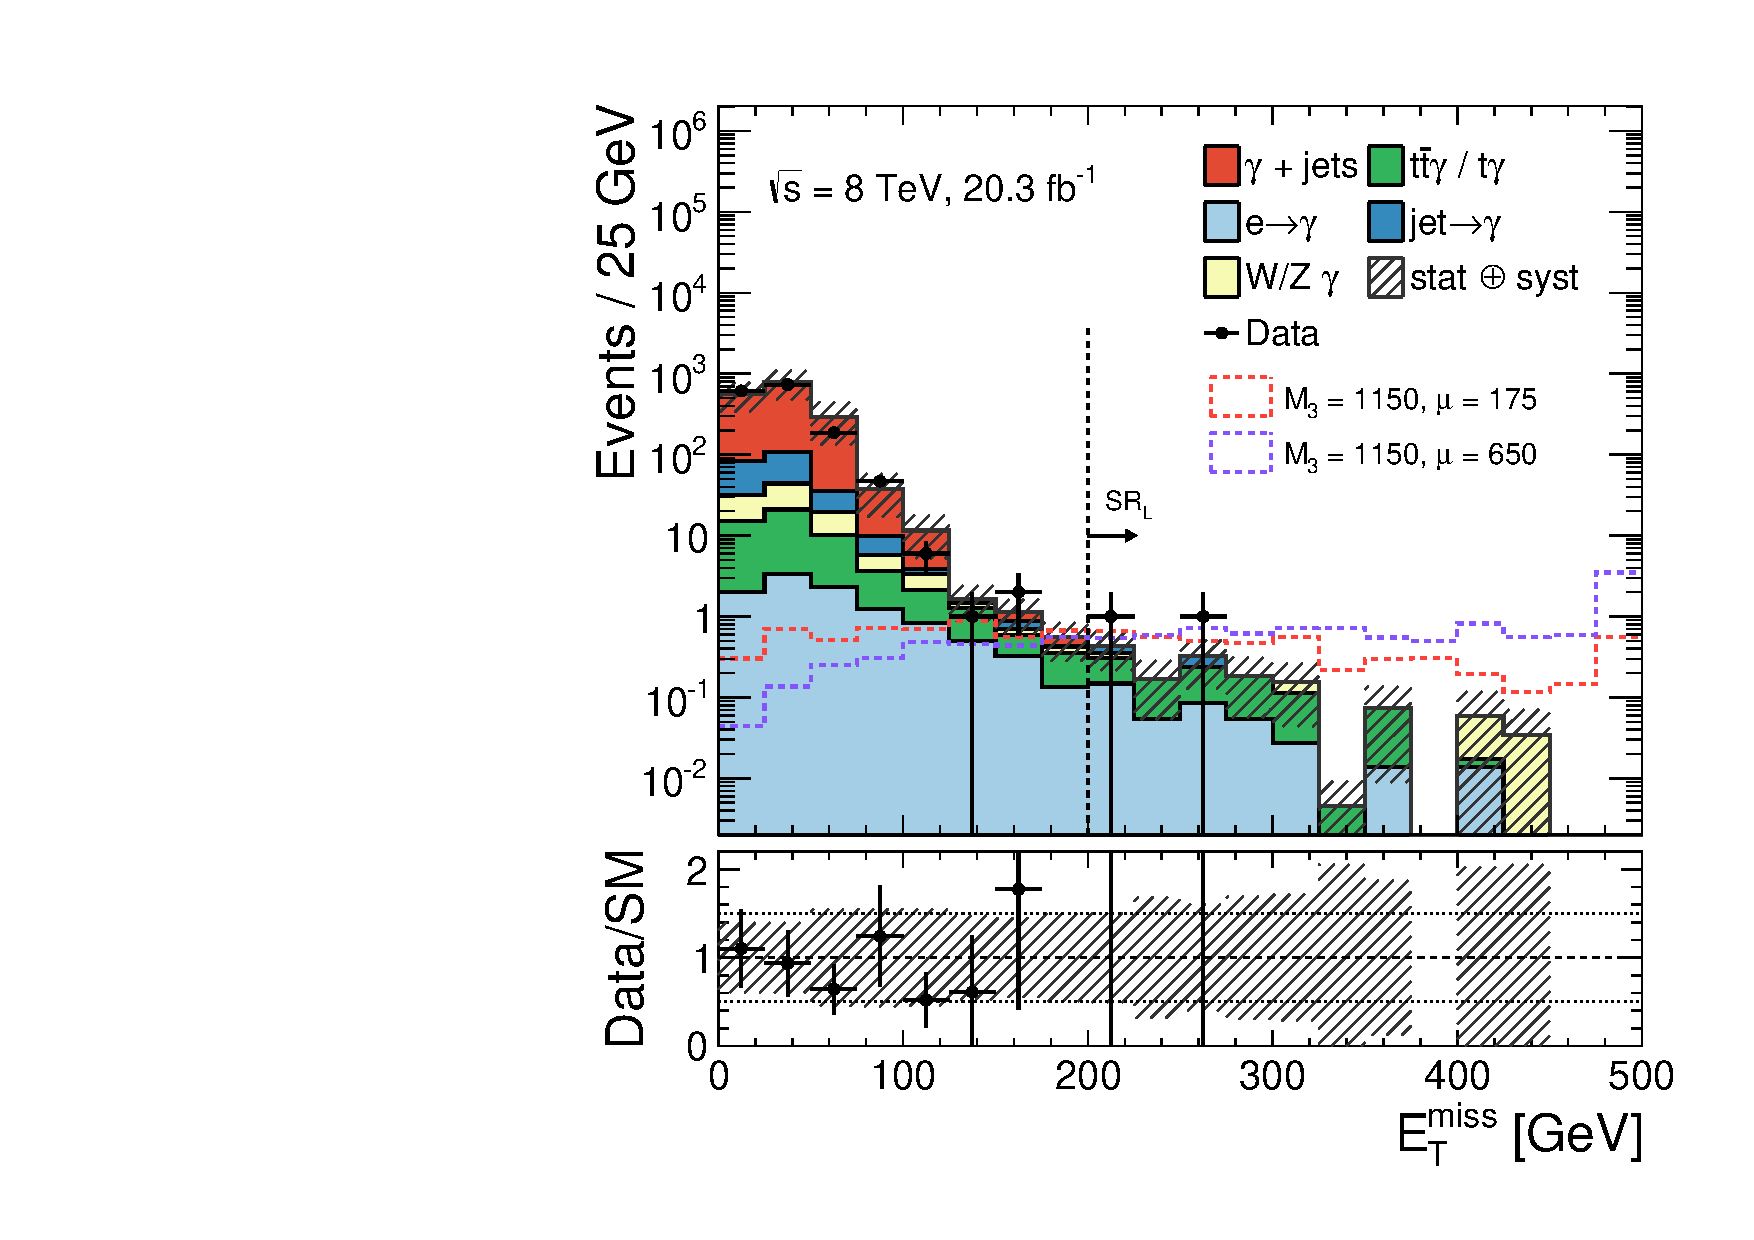
\includegraphics[width=0.49\textwidth]{plot_after_SRL_met_et}
  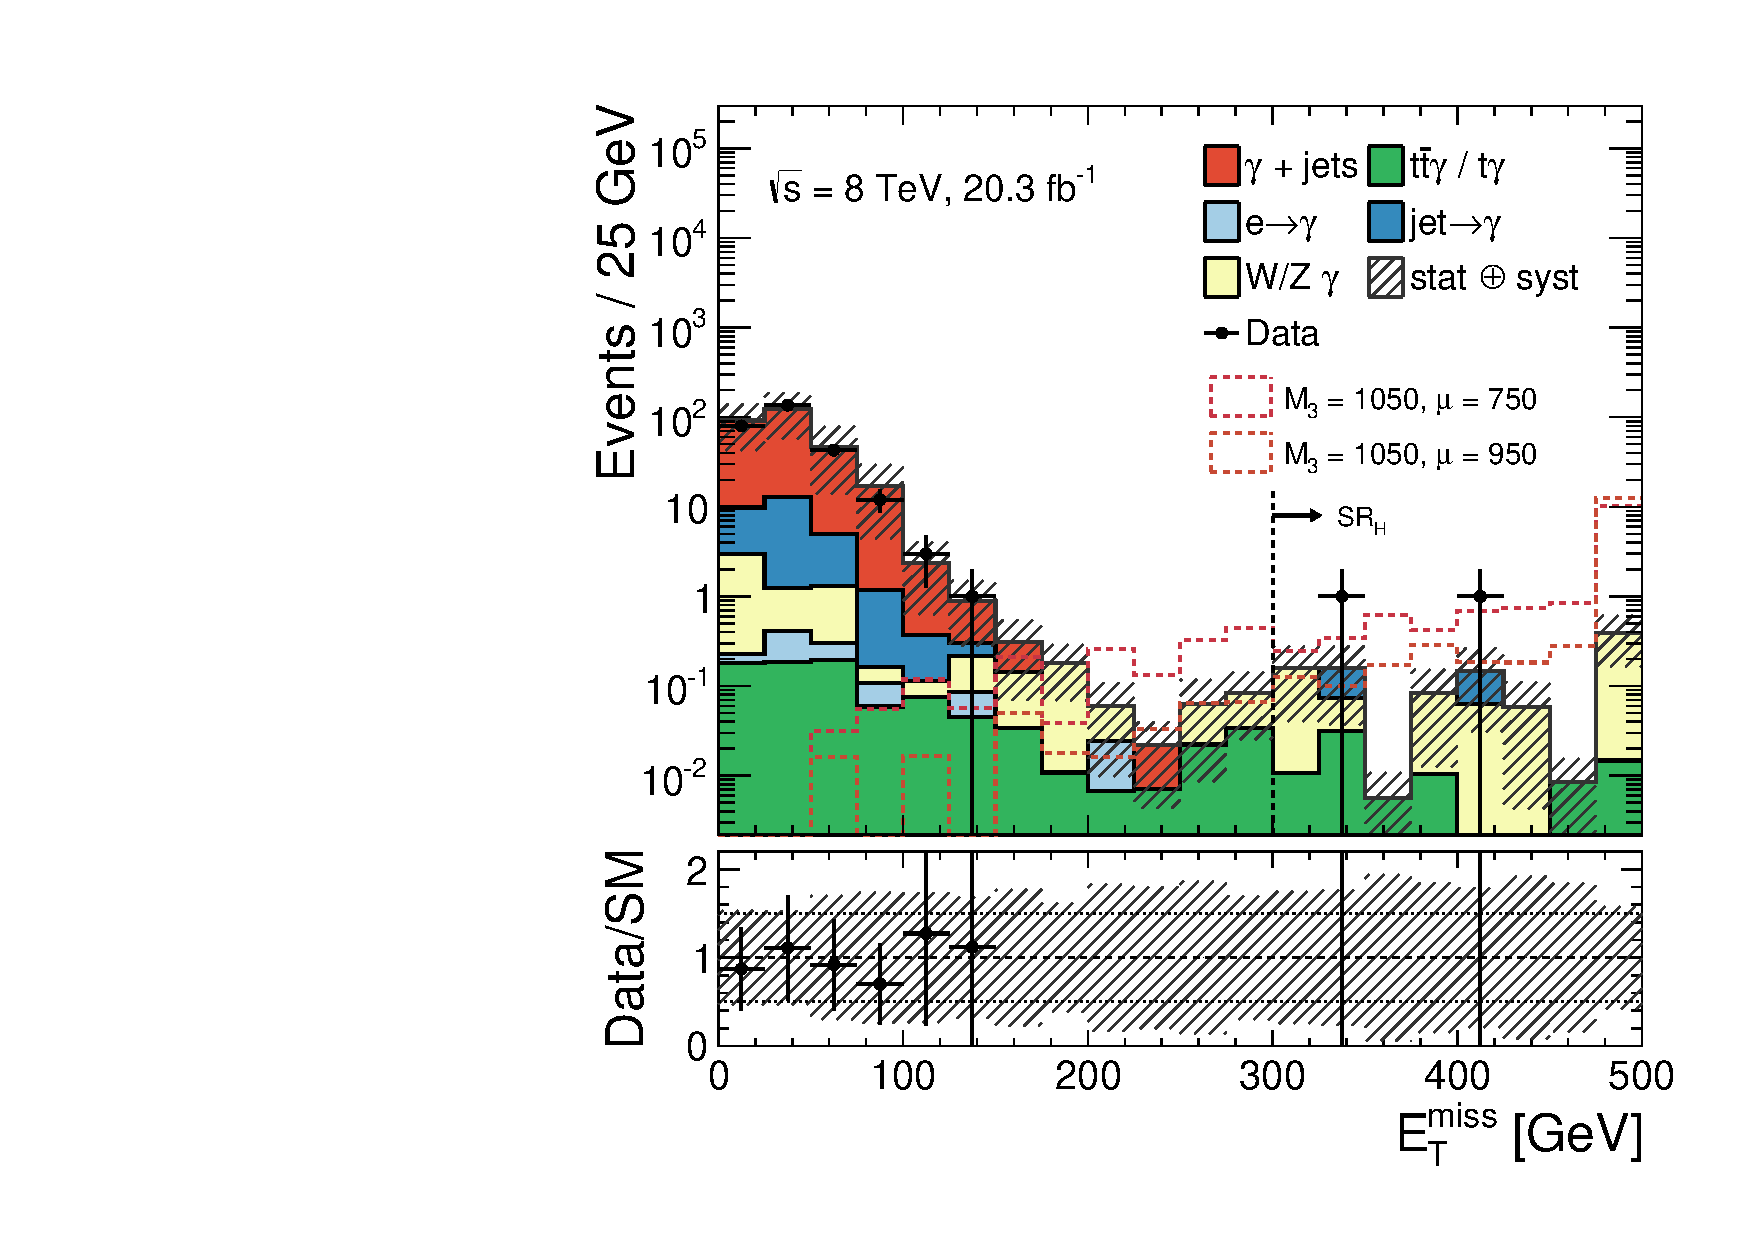
\includegraphics[width=0.49\textwidth]{plot_after_SRH_met_et}

  \caption{Distribución de {\met} comparando datos y el fondo esperado para la selección de la región {\SRL} (izquierda) y {\SRH} (derecha), sin el corte
    en {\met}. La distribución esperada para dos muestras de señal es también graficada para su comparación.}
  \label{fig:met_sr}

\end{figure}


El resumen de los resultados para todas las regiones pueden verse en
\cref{fig:fit_region_composition}.


\begin{figure}[!htbp]
  \centering

  \includegraphics[width=0.8\textwidth]{region_composition_srl}
  \includegraphics[width=0.8\textwidth]{region_composition_srh}

  \caption{Comparación entre el número de eventos observado y esperado en cada
    una de las regiones correspondientes a {\SRL} (arriba) y {\SRH} (abajo).}

  \label{fig:fit_region_composition}

\end{figure}


Las incertezas sistemáticas dominantes en cada SR, en el número total predicho de fondo
se presentan en \cref{tab:fit_result_sr2_syst,tab:fit_result_sr3_syst}.
Debido a que las incertezas individuales pueden estar correlacionadas y las
correlaciones negativas entre normalizaciones (representando el impacto de la
estadística en las CR en la incerteza total), la incerteza total no es
necesariamente la suma en cuadratura de las mismas.
La incerteza estadistica se ilustra con el valor de la raíz cuadrada del número de eventos esperado con
la finalidad de mostrar el impacto relativo de la incerteza estadística con respecto a la
incerteza total del fondo. Las incertezas sistemáticas relativas con respecto a
las predicciones del fondo son grandes, del orden de 54\% (58\%) para {\SRL}
(\SRH). En {\SRL} las incertezas dominantes provienen de la
normalización y de las incertezas teóricas del fondo de {\ttgam}, seguidas por la
incerteza en la escala de energía de los jets y la estadística en la SR. En
{\SRH}, las incertezas están dominadas por las incertezas teóricas del fondo
{\zgam} y {\gjet}, y la incerteza estadística y de normalización del fondo
{\wgam}.

%% Since the individual uncertainties can be correlated and the negative correlations between normalizations (representing the
%% impact of the CR statistics on the total uncertainty) and systematic uncertainties are observed as expected, they
%% do not necessarily add up by quadrature to the total background uncertainty. The square
%% root of the number of the expected events are calculated in order to illustrate the relative impact of the
%% SR Poisson statistical uncertainties with respect to the total background uncertainties. The
%%  relative systematic uncertainties with respect to the background predictions are large, around 54\% (58\%) for SR2 (SR3). In SR2, the main uncertainties
%% after the fit come from the normalisation and the theoretical uncertainties of the \ttbargam\ background, followed by the jet energy scale and the MC statistics
%% in the SR. In SR3, the uncertainties are dominated by the theoretical uncertainties on \zgam and \gjet backgrounds, the MC statistics and the normalisation uncertainties of the \wgamma\ production.

%% Similar breakdown tables but separated on each background prediction in each SR are presented in \Tab \ref{tab:fit_result_sr2_syst_perbkg}-\ref{tab:fit_result_sr3_syst_perbkg}.


\begin{table}[!htbp]
  \centering

  \caption{Resumen de las incertezas sistematicas dominantes en la estimacion del fondo total
    en {\SRL}. Notar que las incertezas individuales pueden estar correlacionados, y la incerteza
    total no es necesariamente la suma en cuadratura de estas. Los porcentajes muestran el tamano
    de la incerteza relativo al fondo esperado total.}
  \label{tab:fit_result_srl_syst}

  \begin{tabularx}{\textwidth}{LR}
\hline
{\bf Incertezas}                                    & {\SRL}            \\
\hline
Eventos esperados SM             &  $1.27$       \\
\hline
Incerteza estadística total $(\sqrt{N_\mathrm{SM}})$              & $\pm 1.13$       \\
Incerteza sistemática total               & $\pm 0.43\ [34.18\%] $             \\
\hline
$\alpha_{\tgam}$         & $\pm 0.36\ [28.0\%] $       \\
$\mu_{T}$         & $\pm 0.35\ [27.7\%] $       \\
$\gamma_\mathrm{SR}$        & $\pm 0.22\ [17.4\%] $       \\
$\alpha_\mathrm{JES}$         & $\pm 0.21\ [16.5\%] $       \\
$\alpha_{\wgam}$         & $\pm 0.09\ [7.3\%] $       \\
$\mu_{W}$        & $\pm 0.08\ [6.7\%] $       \\
$\alpha_{j\to\gamma}$         & $\pm 0.08\ [6.3\%] $       \\
$\alpha_{e\to\gamma}$         & $\pm 0.07\ [5.7\%] $       \\
$\alpha_{\mathrm{JER}}$         & $\pm 0.06\ [4.3\%] $       \\
%% $\alpha_{Z\gamma}$         & $\pm 0.03\ [2.7\%] $       \\
%% $\alpha_\mathrm{EGMAT}$         & $\pm 0.03\ [2.2\%] $       \\
%% $\alpha_\mathrm{EGRES}$         & $\pm 0.03\ [2.0\%] $       \\
%% $\alpha_\mathrm{SCALEST}$         & $\pm 0.02\ [1.7\%] $       \\
%% $\alpha_\mathrm{PRW}$         & $\pm 0.01\ [0.71\%] $       \\
%% $\alpha_\mathrm{RESOST}$         & $\pm 0.00\ [0.35\%] $       \\
%% $\alpha_{t\gamma}$         & $\pm 0.00\ [0.34\%] $       \\
%% $\alpha_\mathrm{PHEFF}$         & $\pm 0.00\ [0.06\%] $       \\
%% $\mu_{Q}$         & $\pm 0.00\ [0.02\%] $       \\
%% $\alpha_{\gamma j}$         & $\pm 0.00\ [0.02\%] $       \\
\hline
\end{tabularx}

\end{table}

\begin{table}[!htbp]
  \centering

  \caption{Resumen de las incertezas sistematicas dominantes en la estimacion del fondo total
    en {\SRH}. Notar que las incertezas individuales pueden estar correlacionados, y la incerteza
    total no es necesariamente la suma en cuadratura de estas. Los porcentajes muestran el tamano
    de la incerteza relativo al fondo esperado total.}
  \label{tab:fit_result_srh_syst}

  \begin{tabularx}{\textwidth}{LR}
\hline
{\bf Incertezas}                                    & {\SRH}            \\
\hline
Eventos esperados SM             &  $0.84$       \\
\noalign{\smallskip}\hline\noalign{\smallskip}
Incerteza estadística total $(\sqrt{N_{\rm SM}})$              & $\pm 0.92$       \\
Incerteza sistemática total               & $\pm 0.38\ [45.27\%] $             \\
\hline
$\alpha_{Z\gamma}$         & $\pm 0.21\ [25.4\%] $       \\
$\alpha_{\wgam}$         & $\pm 0.21\ [25.1\%] $       \\
$\gamma_\mathrm{SR}$         & $\pm 0.20\ [24.3\%] $       \\
$\mu_{W}$         & $\pm 0.17\ [20.5\%] $       \\
$\alpha_\mathrm{PRW}$         & $\pm 0.10\ [11.9\%] $       \\
$\alpha_\mathrm{JFAKE}$         & $\pm 0.08\ [9.5\%] $       \\
$\alpha_\mathrm{EGRES}$         & $\pm 0.05\ [5.8\%] $       \\
$\alpha_\mathrm{JER}$         & $\pm 0.04\ [4.8\%] $       \\
%% $\alpha_\mathrm{RESOST}$         & $\pm 0.04\ [4.5\%] $       \\
%% $\alpha_\mathrm{EGMAT}$         & $\pm 0.04\ [4.5\%] $       \\
%% $\mu_{T}$         & $\pm 0.04\ [4.4\%] $       \\
%% $\alpha_\mathrm{JES}$         & $\pm 0.03\ [4.0\%] $       \\
%% $\alpha_{\tgam}$         & $\pm 0.02\ [1.8\%] $       \\
%% $\alpha_\mathrm{MMS}$         & $\pm 0.01\ [1.3\%] $       \\
%% $\alpha_\mathrm{MID}$         & $\pm 0.01\ [1.3\%] $       \\
%% $\alpha_\mathrm{PHEFF}$         & $\pm 0.00\ [0.40\%] $       \\
%% $\alpha_{t\gamma}$         & $\pm 0.00\ [0.22\%] $       \\
\hline
\end{tabularx}


\end{table}




\begin{figure}[!htbp]
  \centering

  \includegraphics[width=\textwidth]{syst_pull_afterFit_SR2} \\
  \includegraphics[width=\textwidth]{syst_pull_afterFit_SR3}

  \caption{Resumen de los parametros despues del ajuste para {\SRL} (arriba) y {\SRH} (abajo).}
  \label{fig:fit_unc_nuisance_SR}

\end{figure}

\begin{figure}[!htbp]
  \centering

  \includegraphics[width=\textwidth]{corr_matrix_srl} \\
  \includegraphics[width=\textwidth]{corr_matrix_srh} \\

  \caption{Matriz de correlacion de los parametros del ajuste, correspondientes a {\SRL} (arriba) y {\SRH} (abajo).}
  \label{fig:fit_corr_SR}

\end{figure}



\subsection{Eventos en las regiones de señal}

Como se mostró en la \cref{tab:bkgfit_sr}, se observaron dos eventos que pasan la selección de cada una de las regiones de
señal.
Un esquema del detector y las senales dejadas por los distintos objetos en el mismo puede verse en las
\cref{fig:evdisplay_sr2_1,fig:evdisplay_sr2_2} para los eventos en la {\SRL} y en las
\cref{fig:evdisplay_sr3_1,fig:evdisplay_sr3_2} para los eventos en la {\SRH}.

Aca explicar que significan cada cosa del plot...


Las visualizaciones
de los eventos es generada con \textsc{Atlantis}\cite{atlantis}.


\begin{figure}[!htbp]
  \begin{center}

    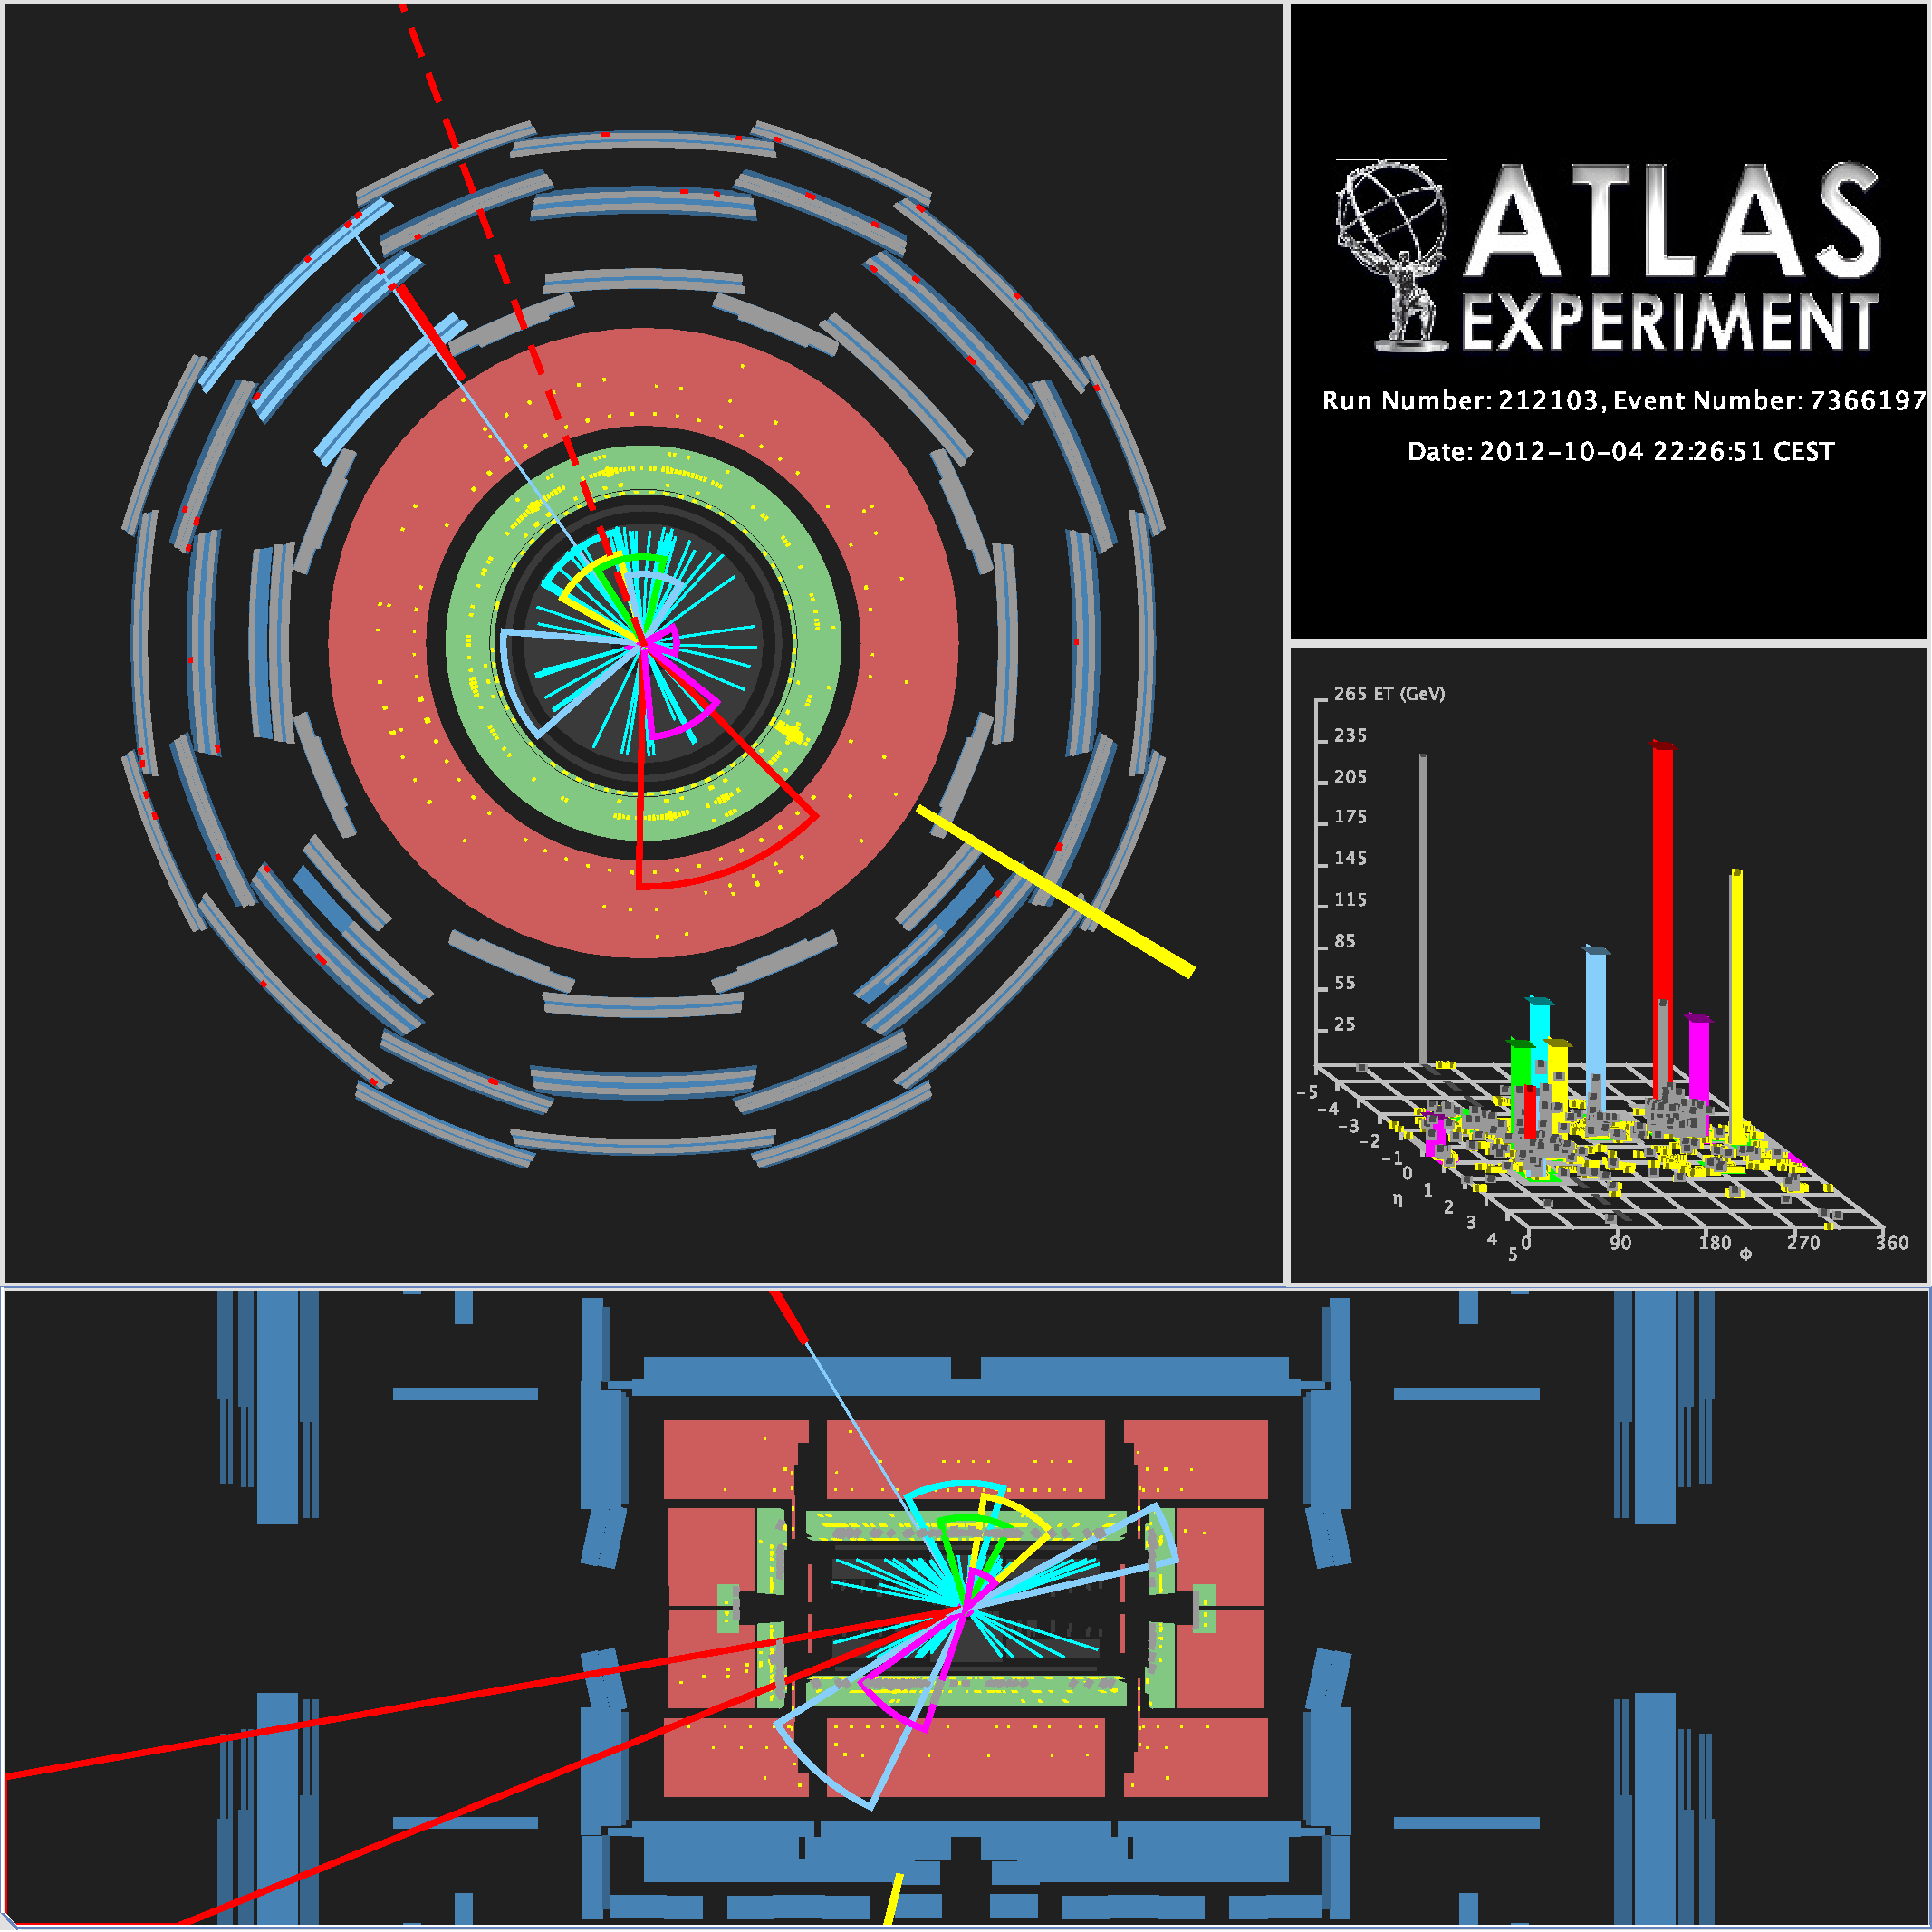
\includegraphics[height=0.45\textheight]{EvtDisplay_212103_73661974}

    \vspace{1cm}

    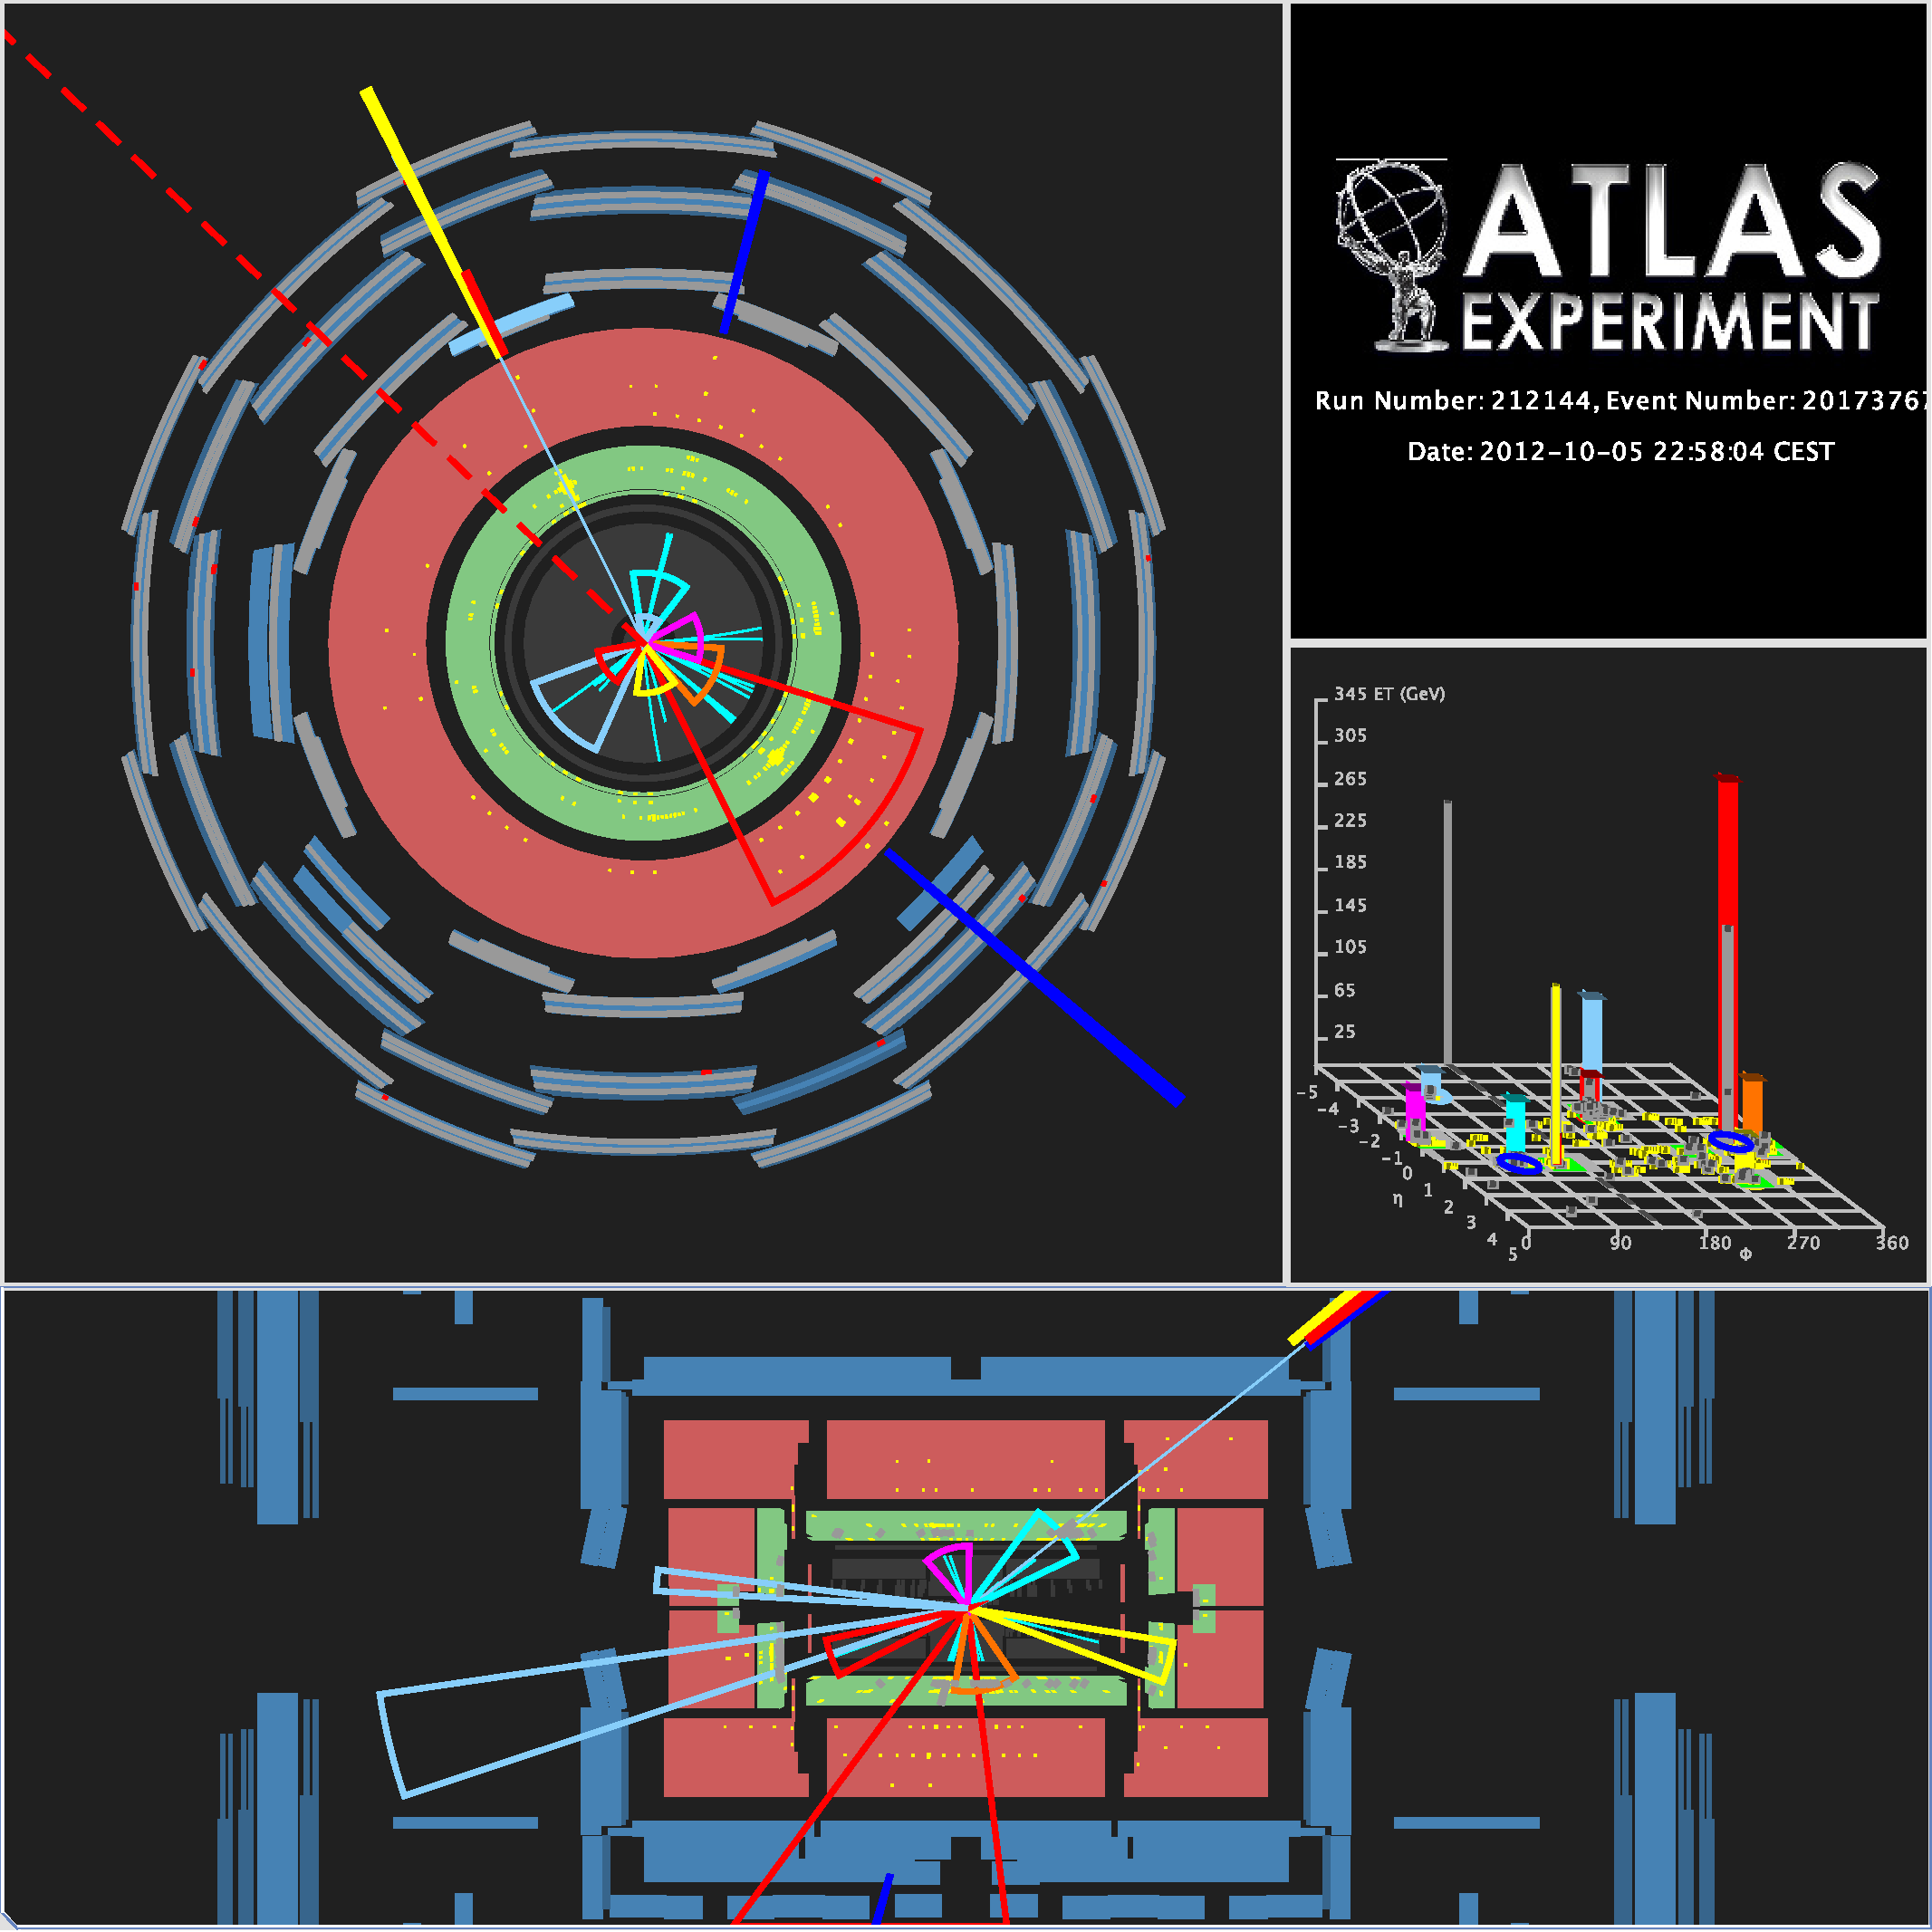
\includegraphics[height=0.45\textheight]{EvtDisplay_212144_201737678}

    \caption{Visualización de uno de los eventos que sobreviven la selección de {\SRL}. Ver detalles en el texto.} %%. Run 212103, Evento 73661974.}
    \label{fig:evdisplay_sr2_1}
  \end{center}
\end{figure}

%% \begin{figure}[!htbp]
%%   \begin{center}
%%   \caption{Visualización de uno de los eventos que sobreviven la selección de {\SRL}. Run 212144, Evento 201737678.}
%%   \label{fig:evdisplay_sr2_2}
%%   \end{center}
%% \end{figure}

\begin{figure}[!htbp]
  \begin{center}

    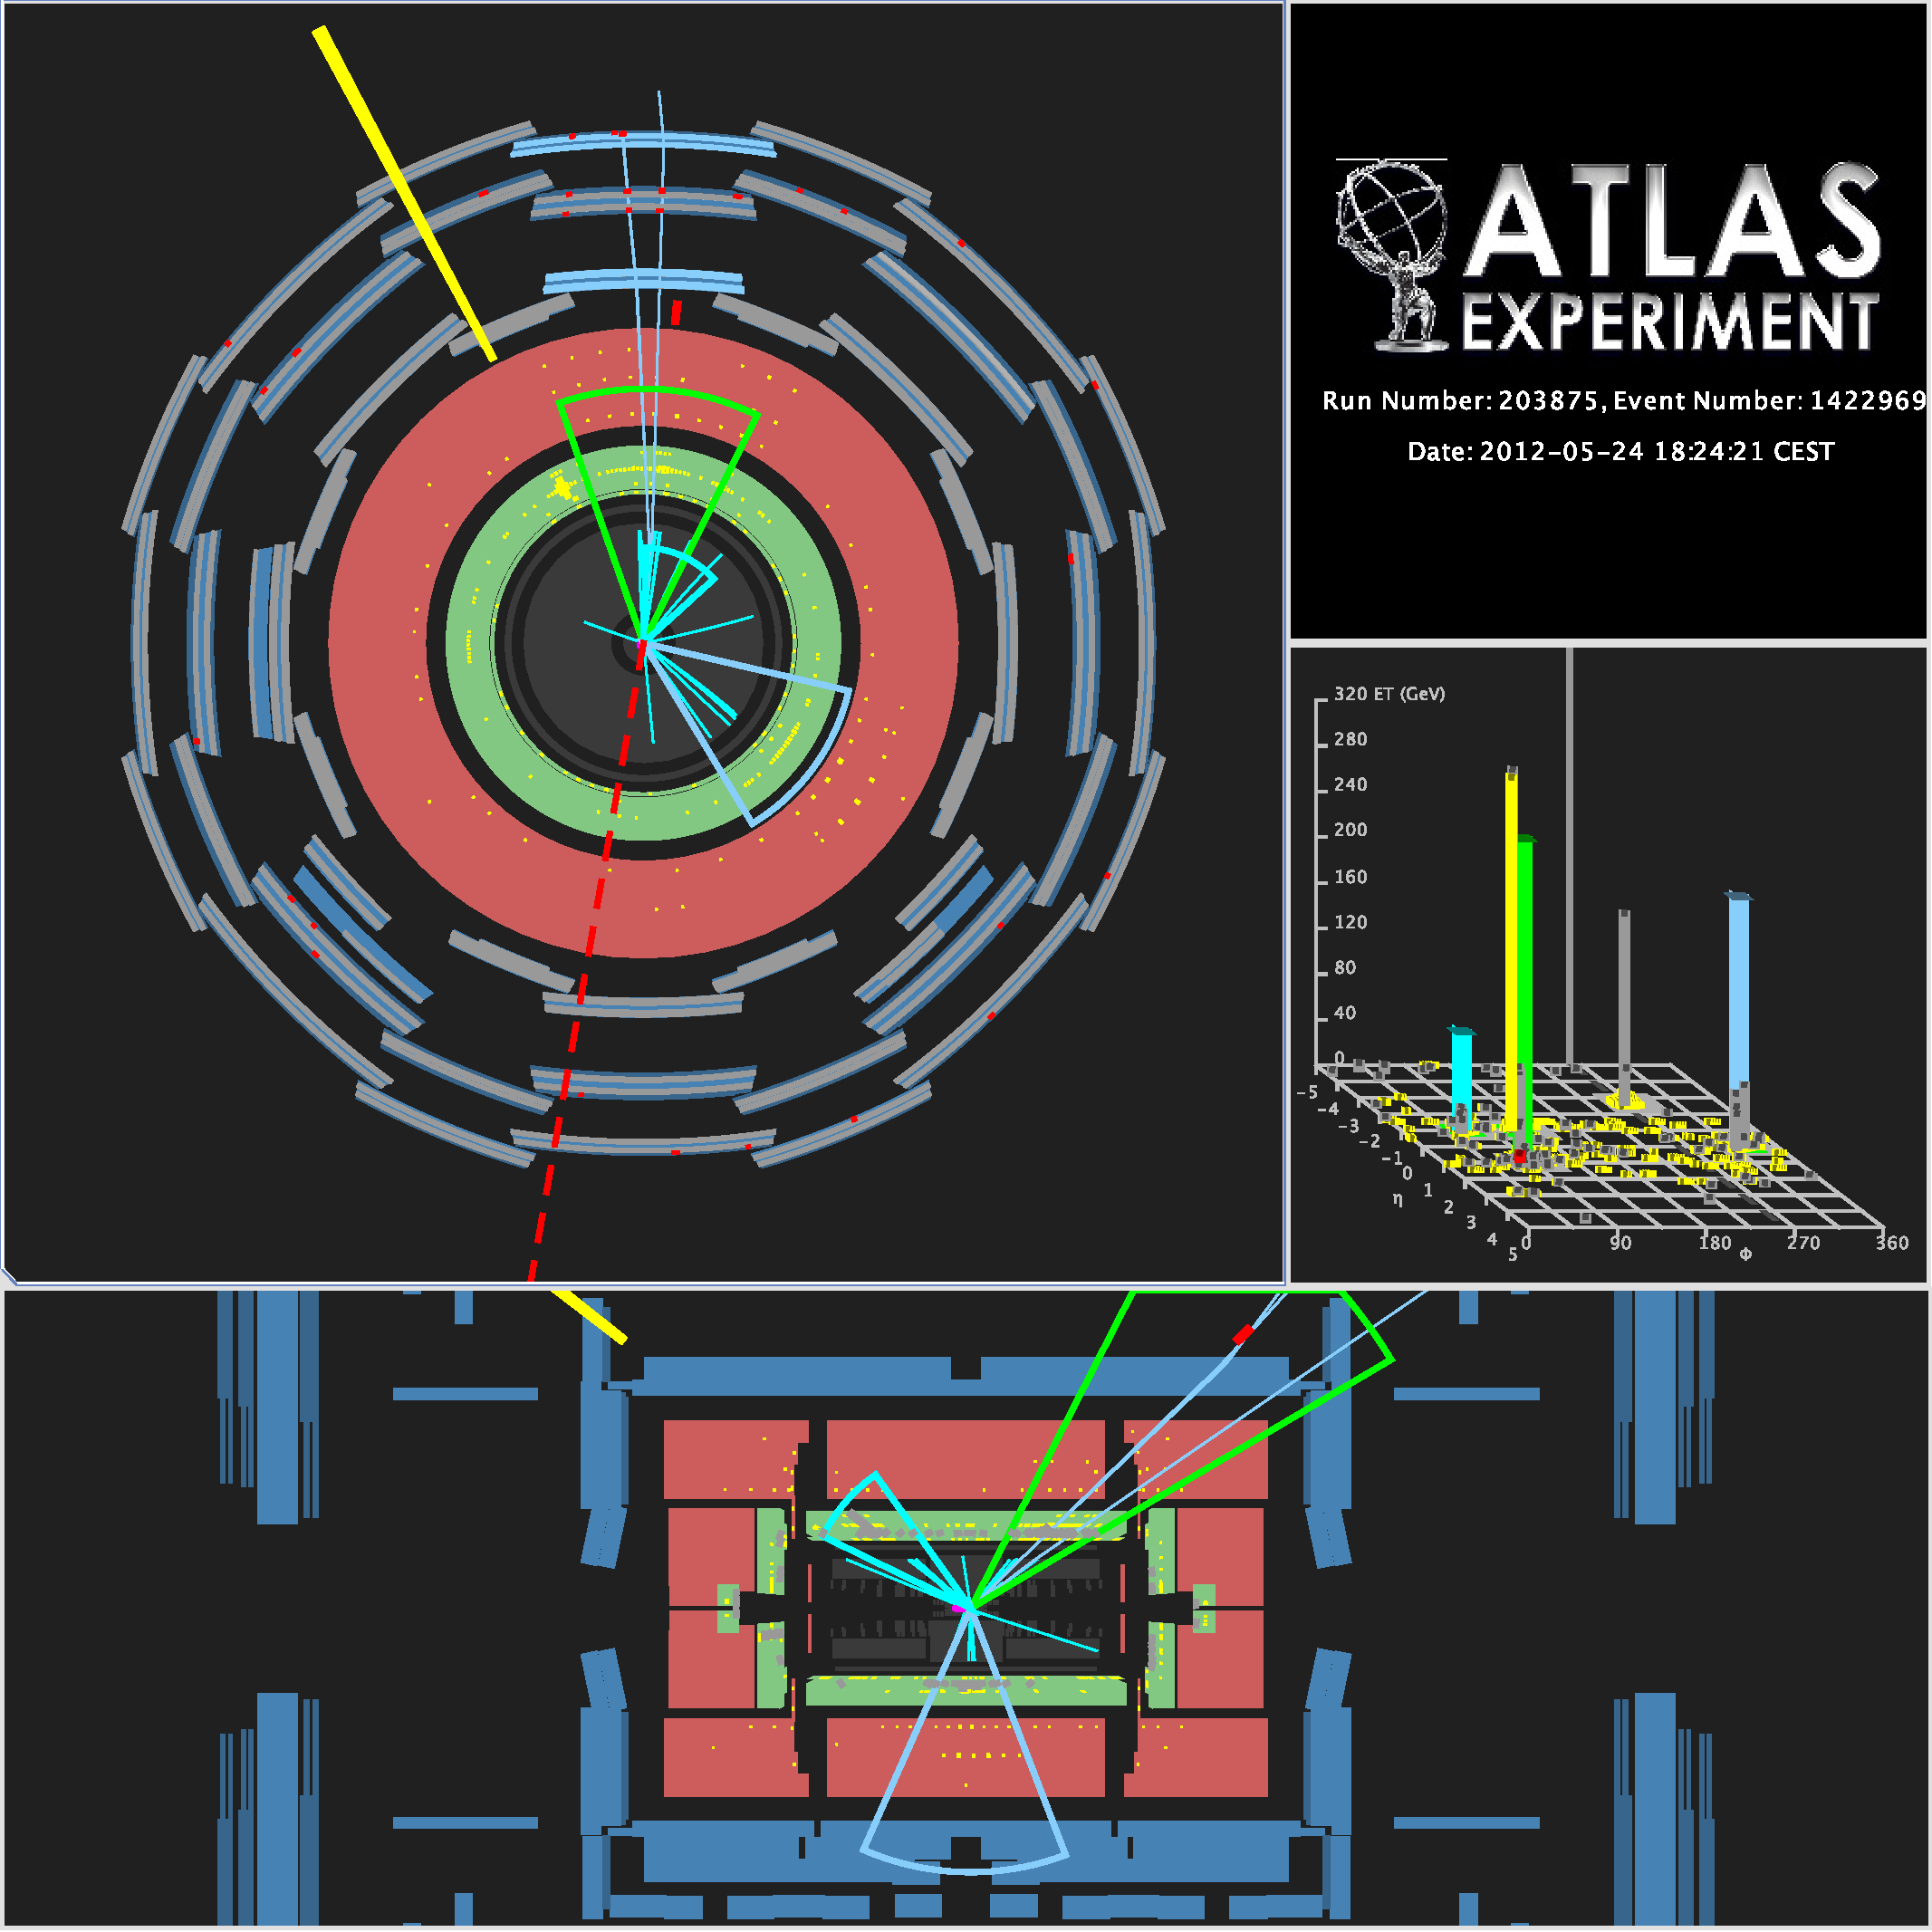
\includegraphics[height=0.45\textheight]{EvtDisplay_203875_14229699}

    \vspace{1cm}

    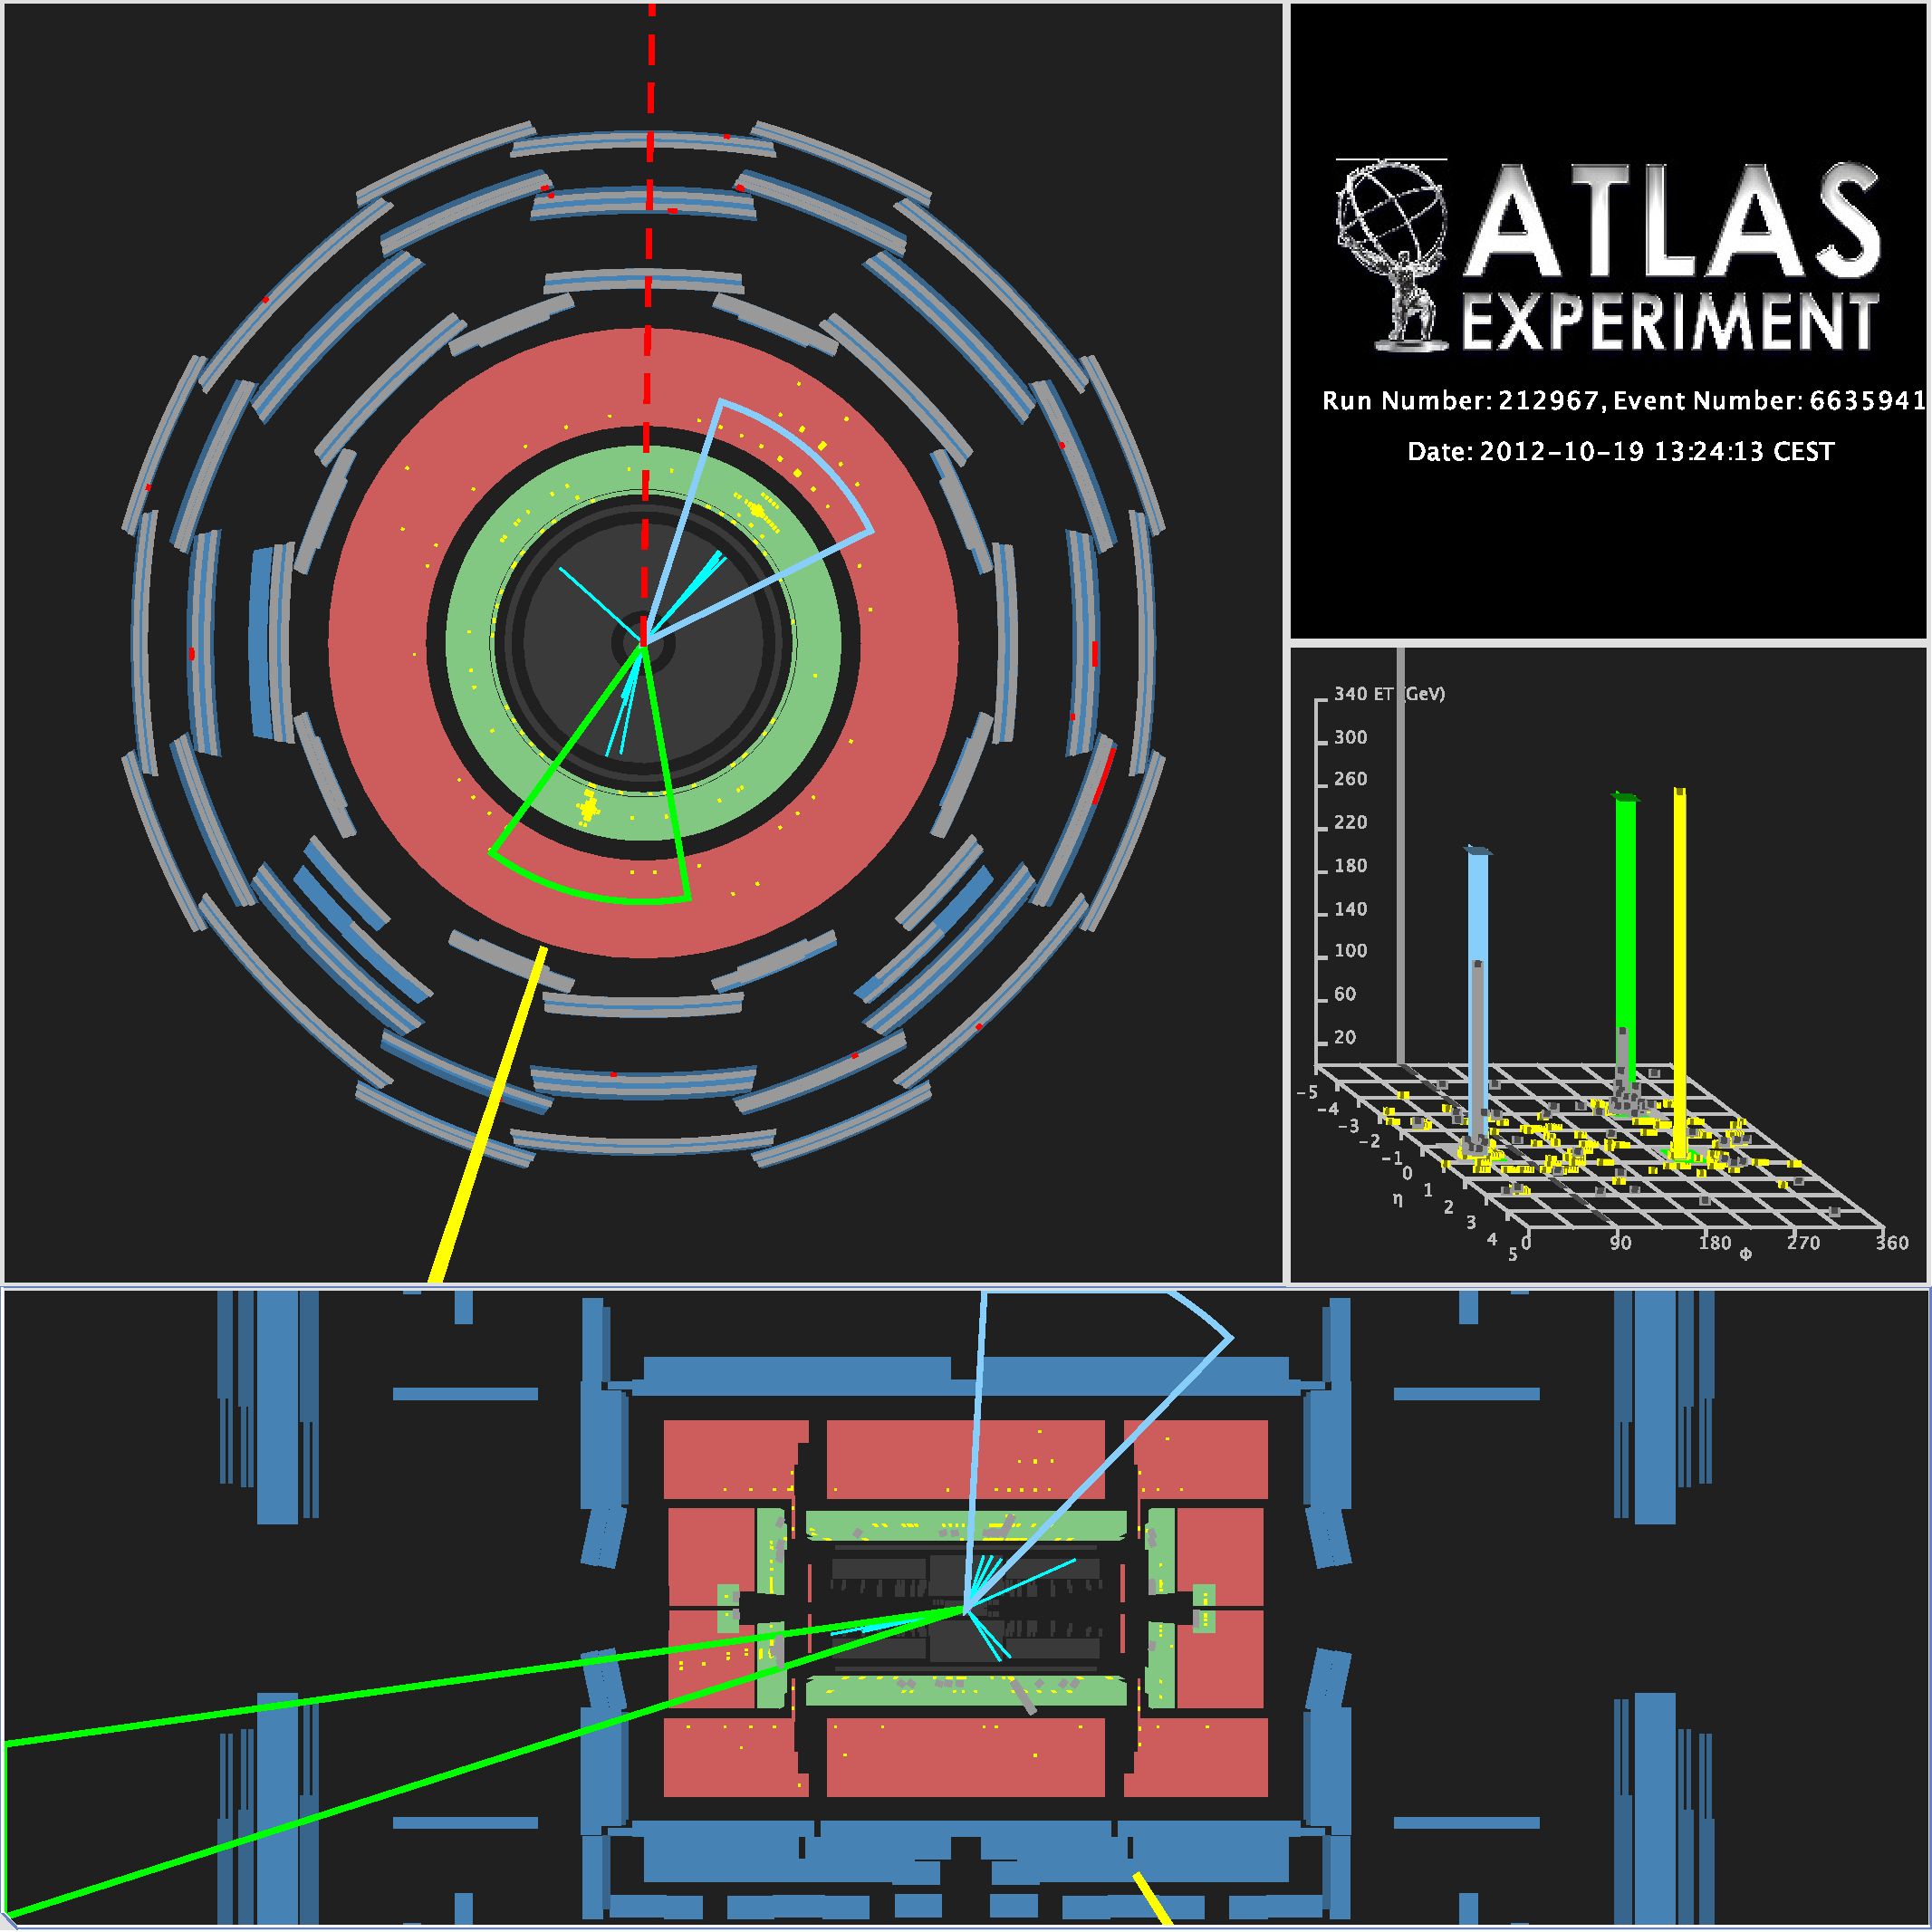
\includegraphics[height=0.45\textheight]{EvtDisplay_212967_66359411}

  \caption{Visualización de los eventos que sobreviven la selección de {\SRH}. Ver detalles en el texto.} %%. Run 203875, Evento 14229699.}
  \label{fig:evdisplay_sr3_1}
  \end{center}
\end{figure}


%% \clearpage


%-------------------------
% SUSY Exclusion limit
%-------------------------
\section{Límites de exclusión en el modelo de SUSY considerado}

Debido a que no se observa un exceso significativo por encima del fondo esperado
del {\SM} en las regiones de señal, se obtuvieron los límites de exclusión en el
modelo de SUSY considerado. Los límites superiores son obtenidos utilizando el
método del {\cls} descripto en la \cref{sec:limits}. Estos límites son
calculados para la sección eficaz nominal del modelo y también con una sección
eficaz de $\pm 1 \sigma$ en la incerteza teórica, siguiendo la recomendación de
ATLAS y el acuerdo de los experimentos del LHC para presentar los resultados.

La \cref{fig:limit_srs} muestra los límites de exclusión esperados y
observados para las dos SR de forma separada. Los límites fueron obtenidos
utilizando $\sim 20000$ pseudo-experimentos. La linea punteada azul muestra el
límite esperado a 95\% CL, con las bandas amarillas indicando la desviación a
1$\sigma$ teniendo en cuenta las incertezas teóricas y experimentales. Los
límites observados están indicados por las lineas en rojo oscuro, donde la linea
solida representa el límite nominal y las lineas punteadas representan el límite
para las variaciones de la sección eficaz de la señal debido a la incerteza
teórica en la misma.

Por diseño, la {\SRL} es importante en la zona de neutralinos livianos, mientras que
la {\SRH} cubre la región mas comprimida del espacio de fases. En la
\cref{fig:limit_combined}, se muestra el límite combinando ambas
regiones de señal, eligiendo en cada punto la que provee el mejor límite.


\begin{figure}[!htbp]
  \centering

  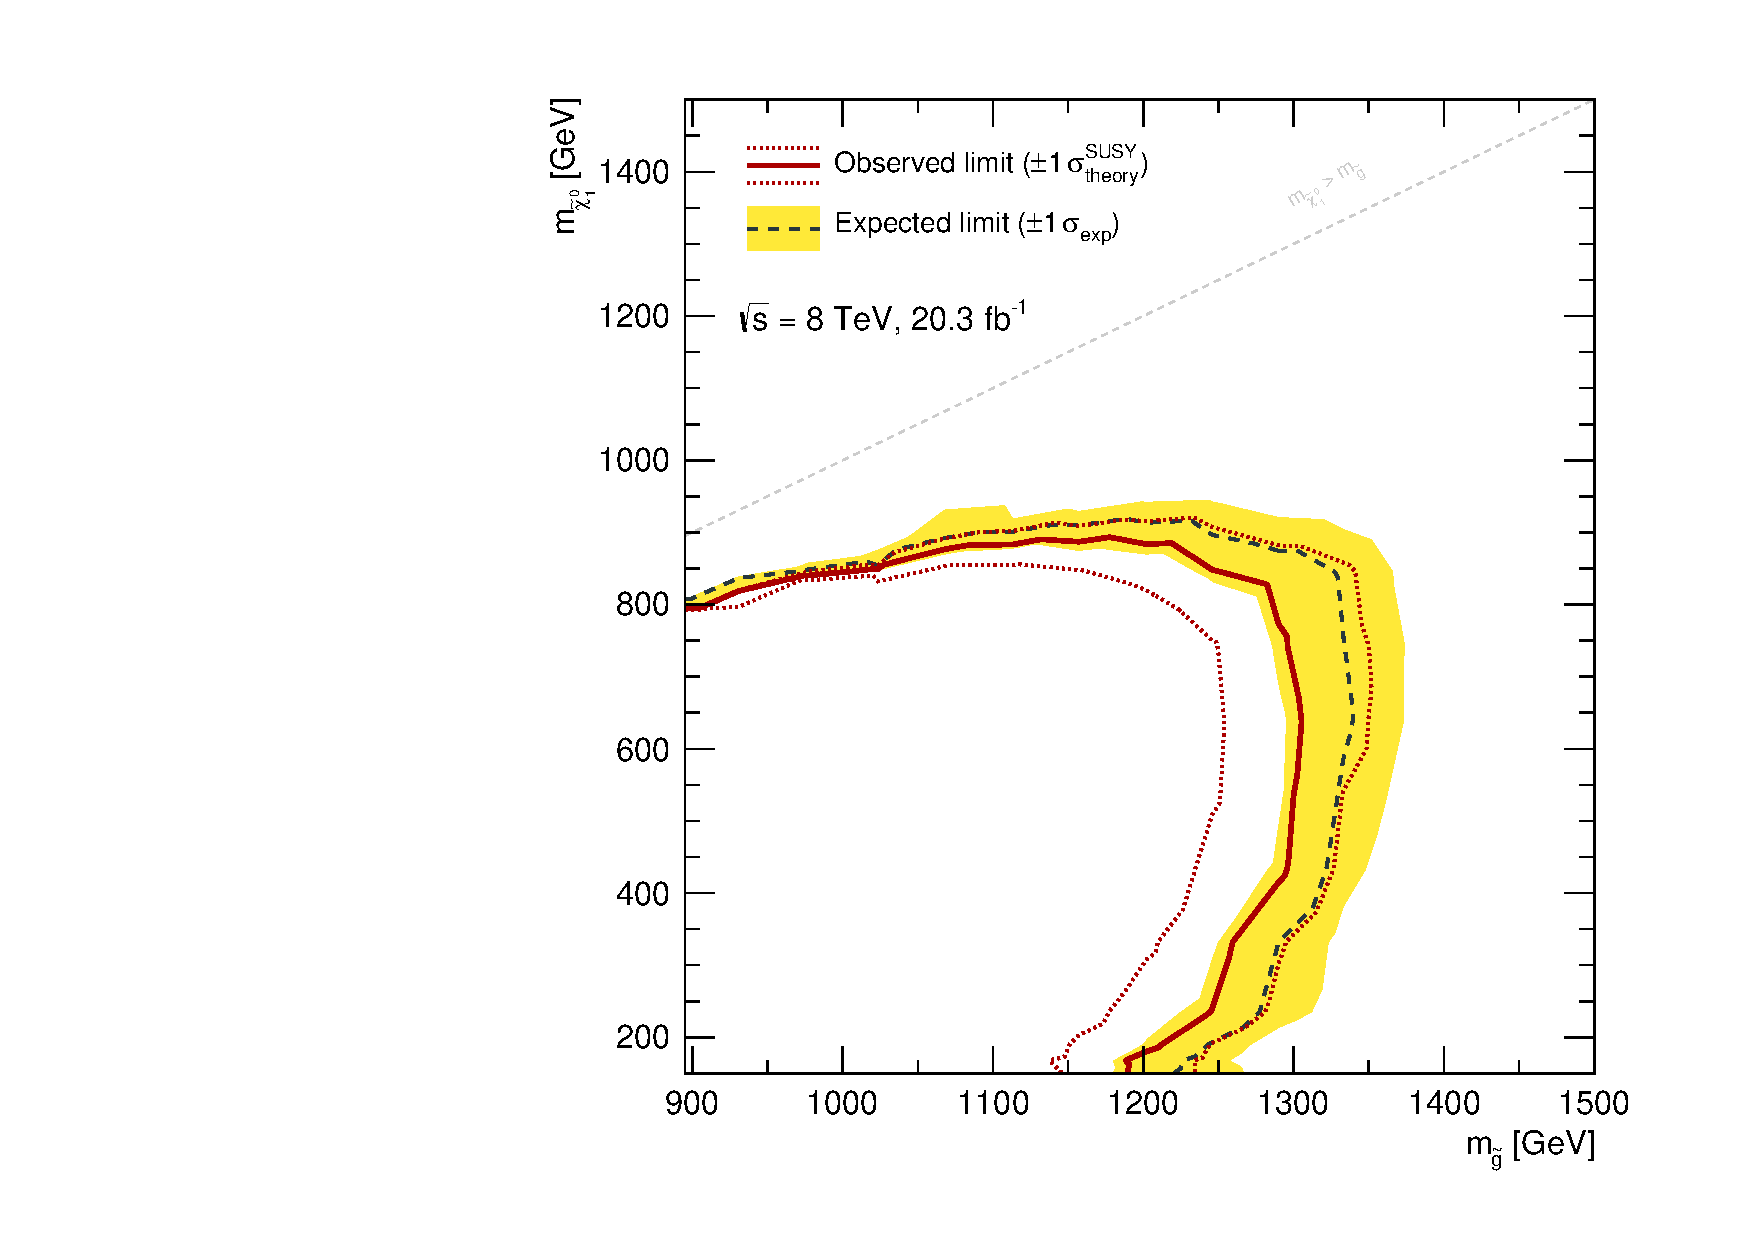
\includegraphics[width=0.49\textwidth]{limitplot_srl}
  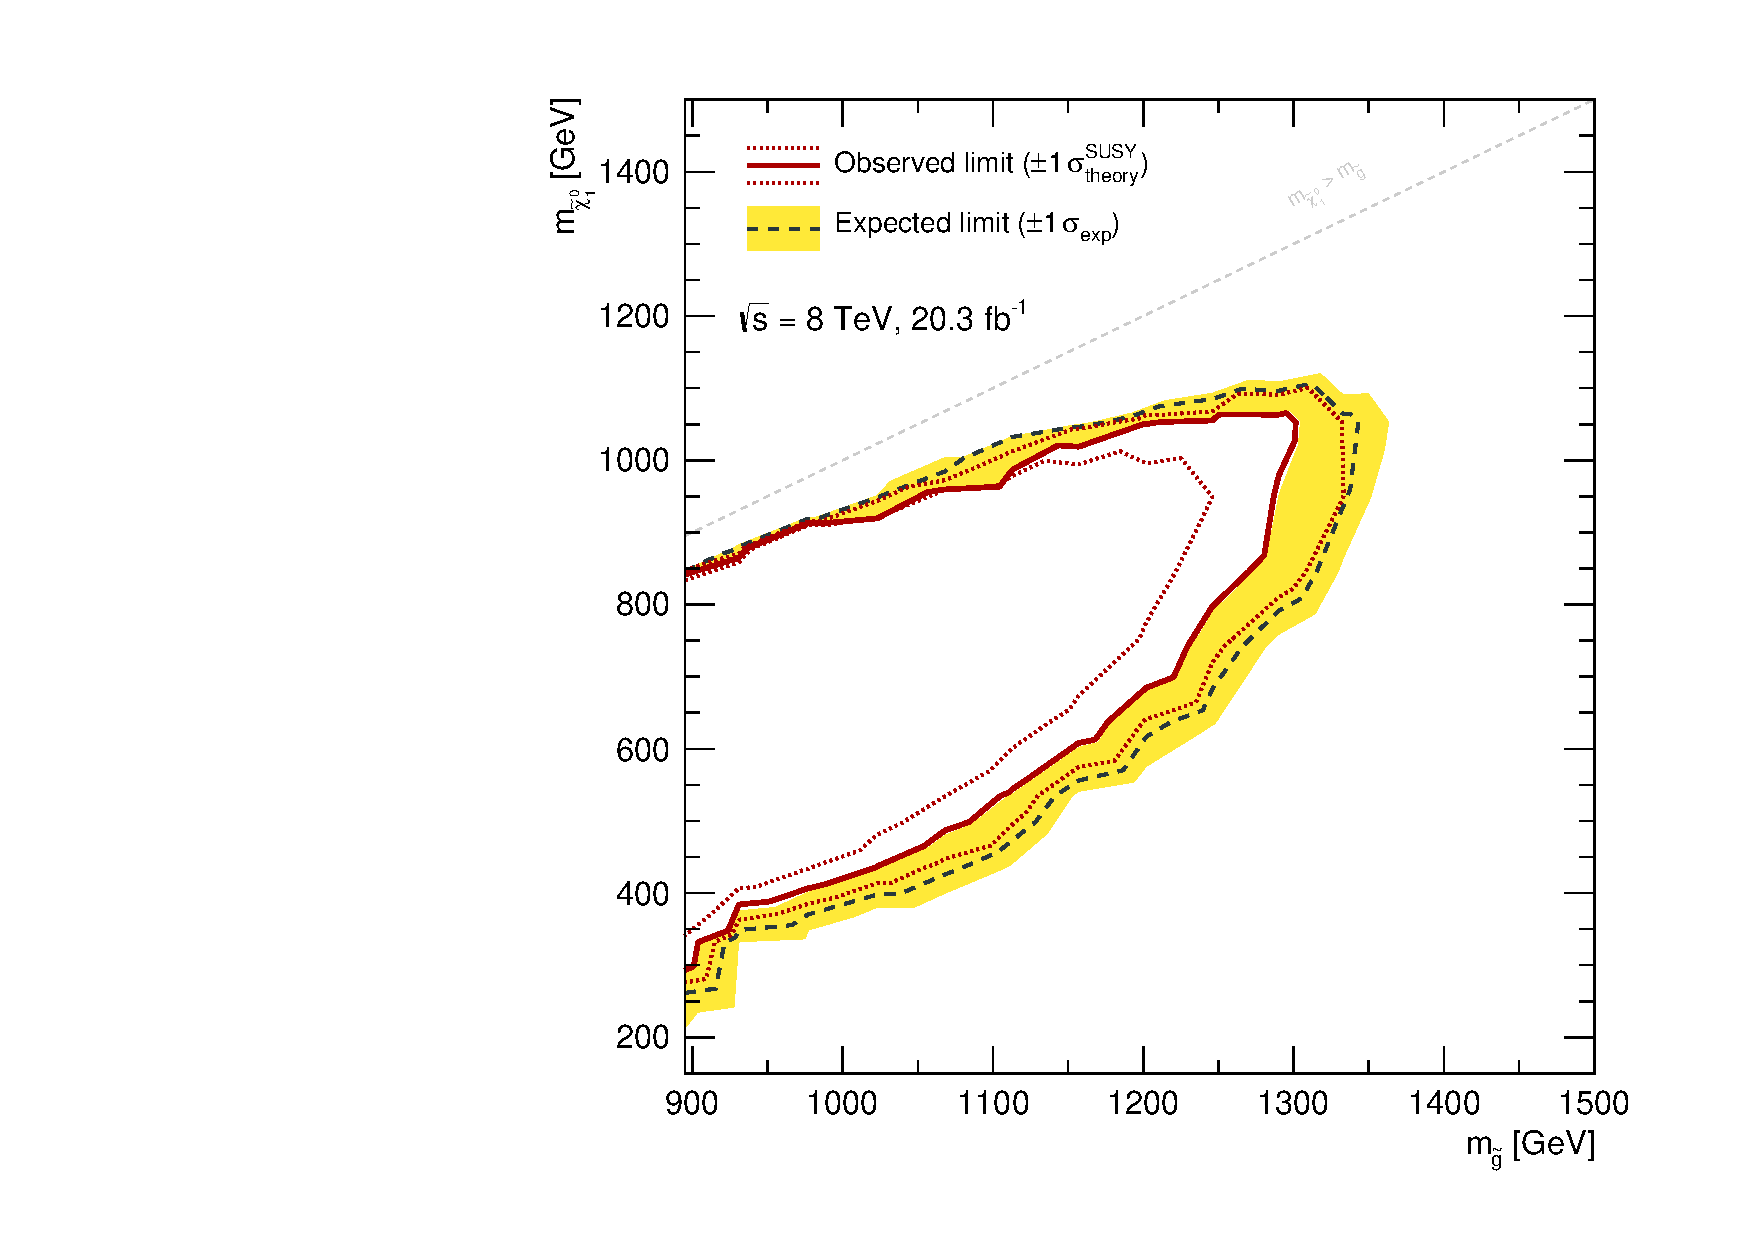
\includegraphics[width=0.49\textwidth]{limitplot_srh}

  \caption{Límites de exclusión a 95\% CL para {\SRL}  (izquierda) y {\SRH} (derecha).}
  \label{fig:limit_srs}
\end{figure}


\begin{figure}[!htbp]
  \centering

  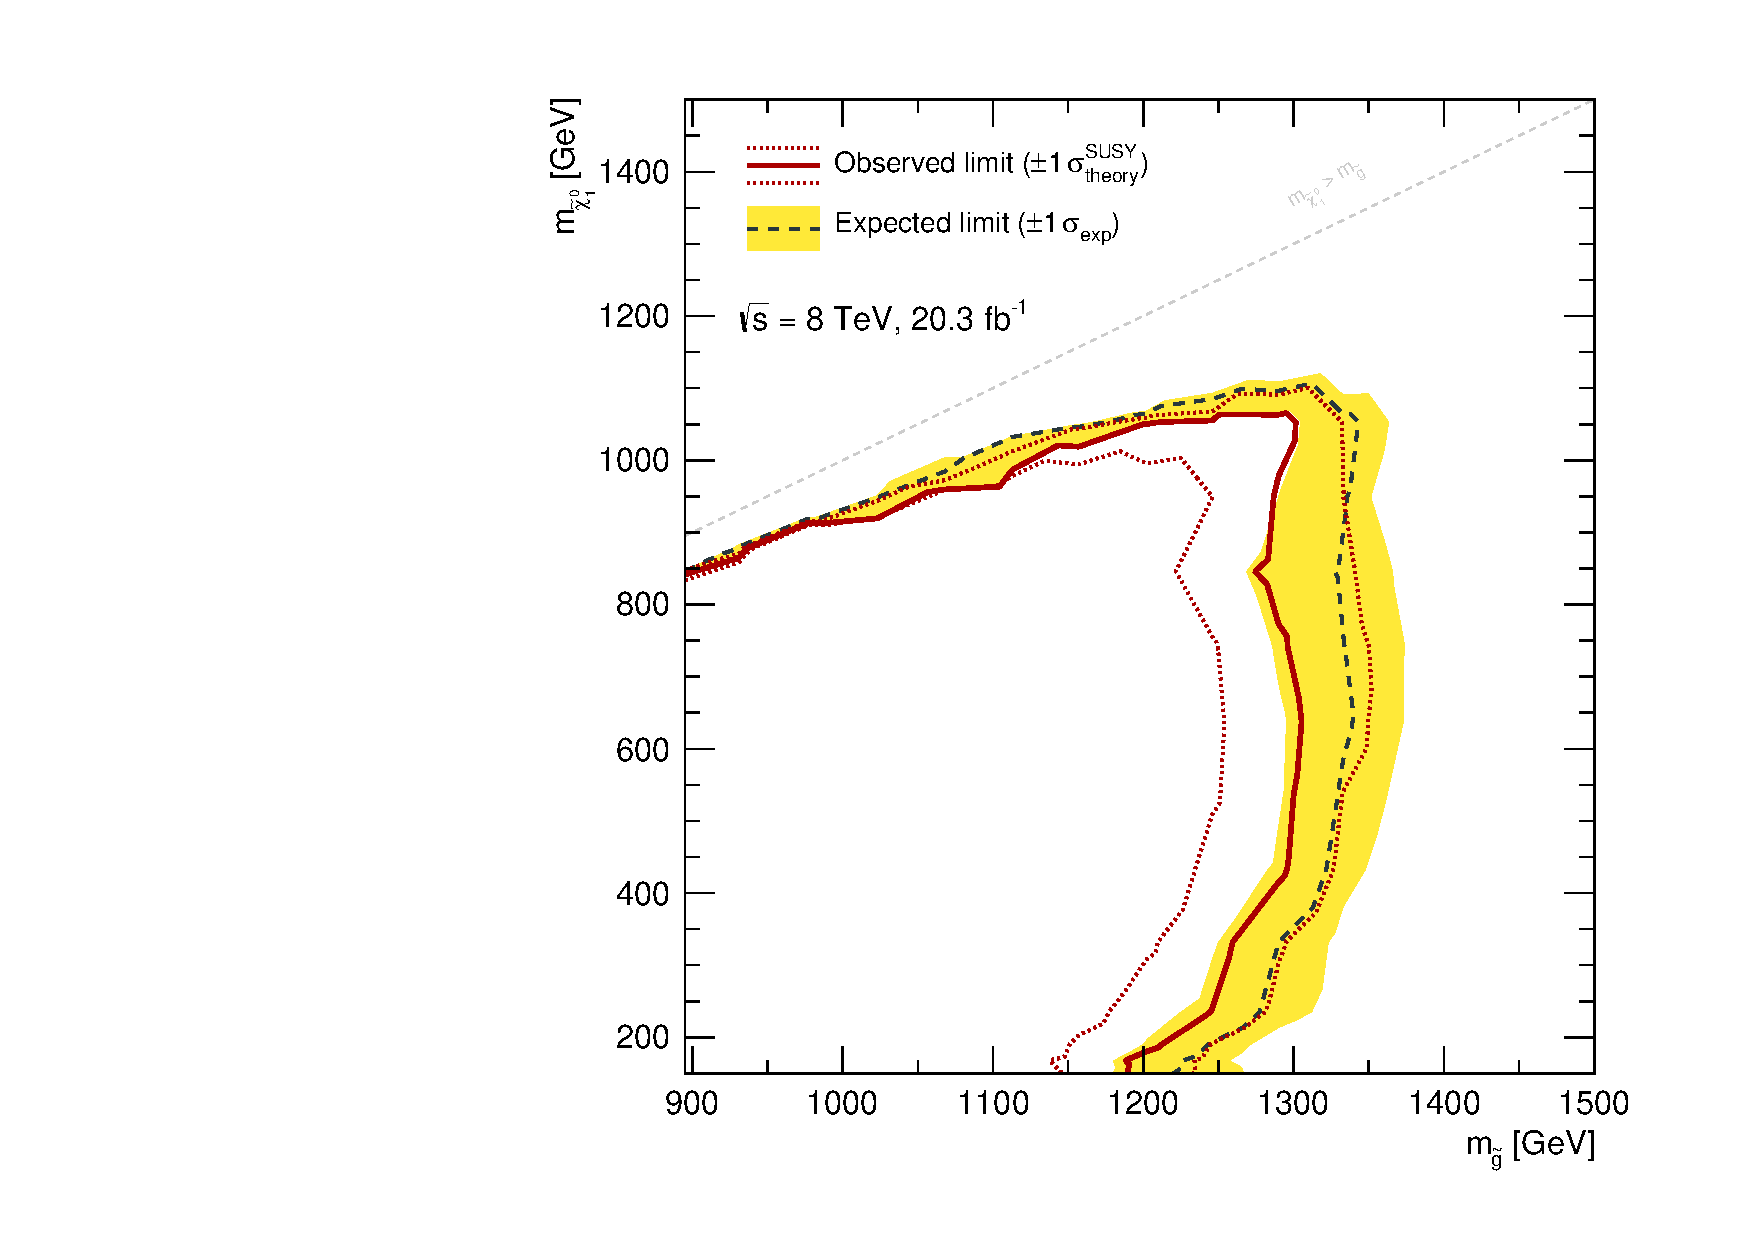
\includegraphics[width=0.8\textwidth]{limitplot_combined}

  \caption{Límites de exclusión para {\SRL} y {\SRH} combinados.
    Los límites son obtenidos usando la región de señal con mejor sensibilidad
    en cada punto.
    La linea punteada azul muestra el límite esperado a 95\% CL, con las bandas amarillas indicando la desviación a
    $1\sigma$ que tiene en cuenta las incertezas teóricas y experimentales. Los
    límites observados están indicados por las lineas en rojo oscuro, donde la línea
    solida representa el límite nominal y las líneas punteadas representan el límite
    para las variaciones de la sección eficaz de la señal debido a la incerteza
    teórica en la misma.}
   \label{fig:limit_combined}

\end{figure}


Como se ve de los graficos, la produccion de gluino es excluida a 95\% {\cl} para
una masa minima (maxima) de 1190 (1320) \gev, para $m_{\ninoone}<{840}\gev$.
Para masas de gluino menores a $1\tev$, un neutralino NLSP es excluido entre
$150\gev$ y $m_{\gluino}-m_{\ninoone}>50\gev$. \note{Tiene sentido esto? Capaz mejor el
número que usamos para el summar plot.}

Hacer referencia al summary plot...


\begin{figure}[!htbp]
  \centering

  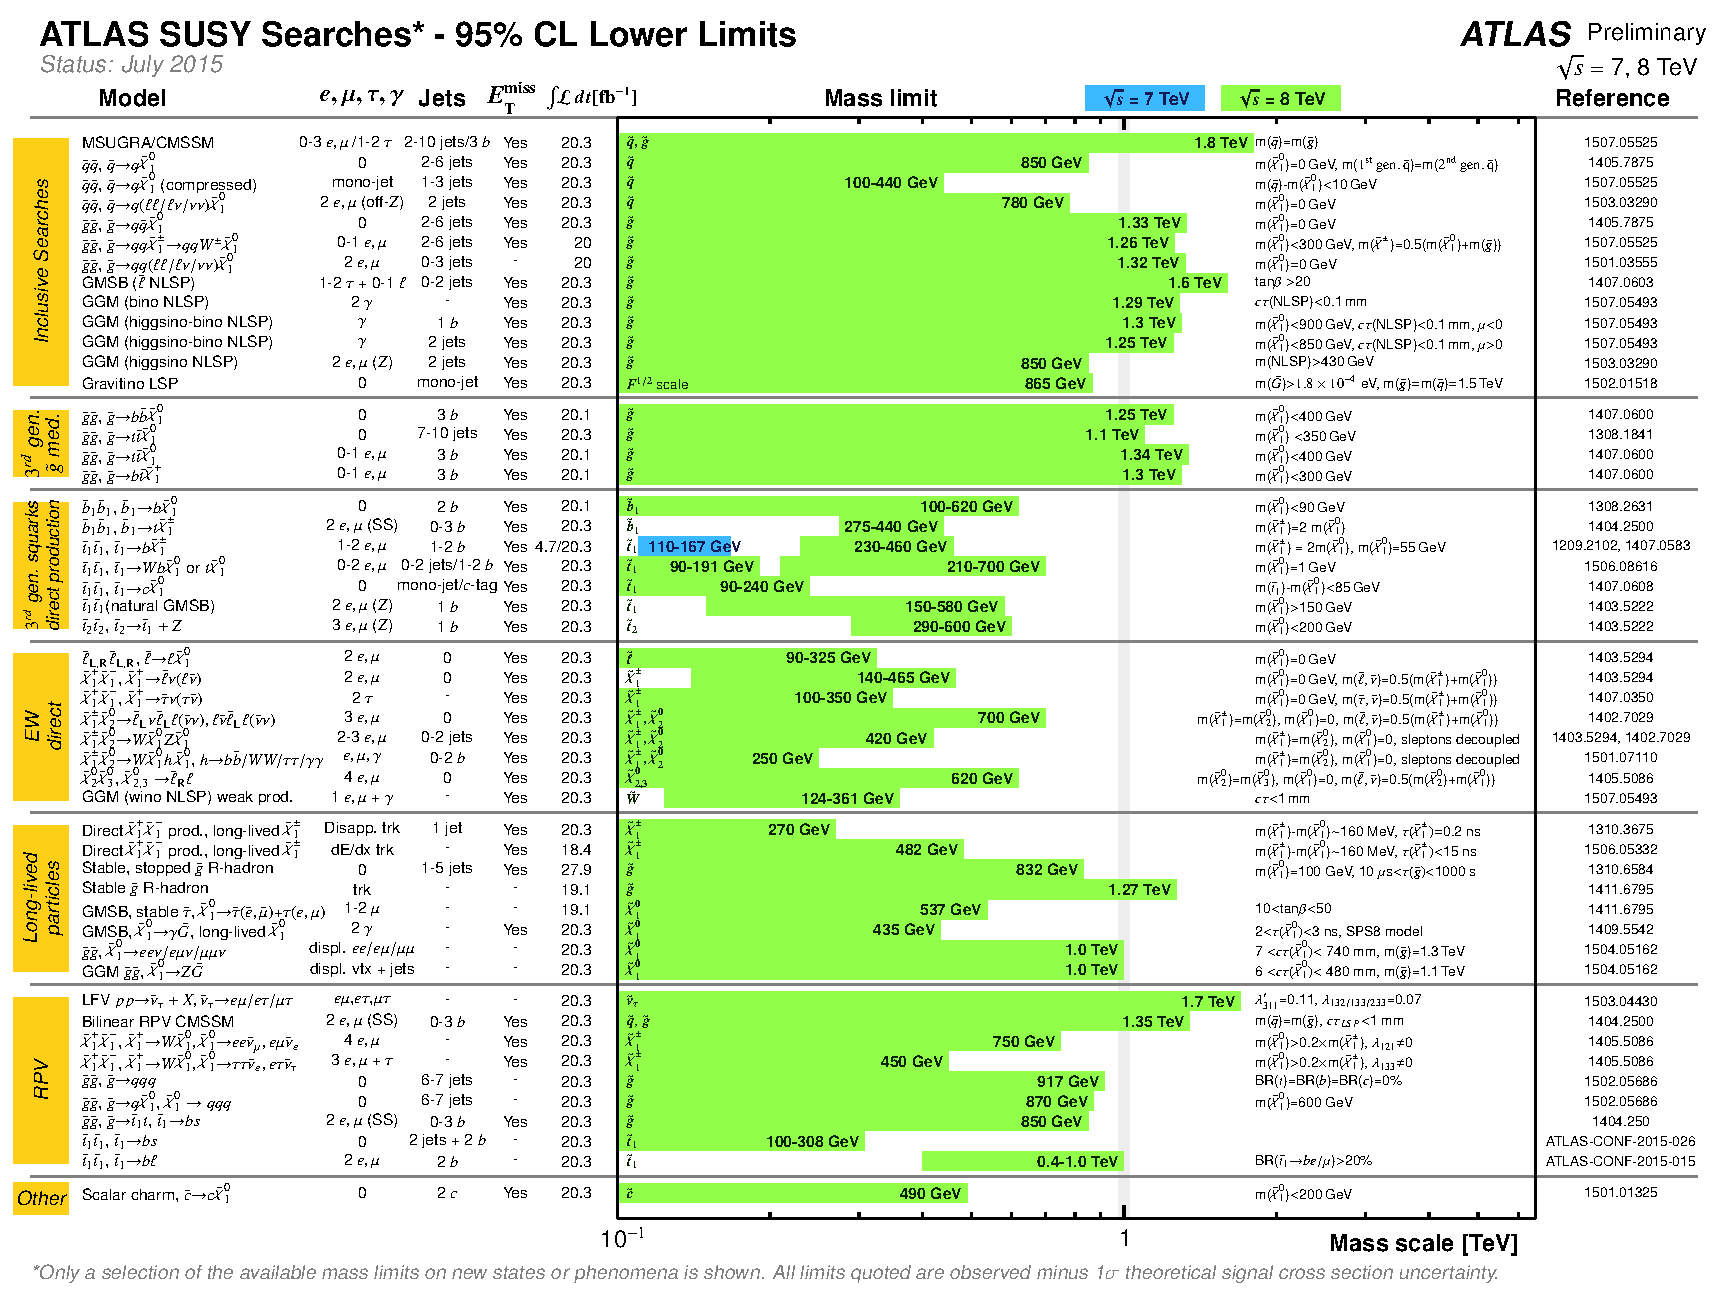
\includegraphics[width=\textwidth]{atlas_susy_run1_summary}

  \caption{Resumen de los límites de exclusion en la masa de las particulas supersimetricas por distintos analisis realizados en ATLAS.
    Solo una seleccion representativa de los resultados dispobibles es mostrada\cite{susy_summary}.}
  \label{fig:susy_summary}

\end{figure}



%-------------------------
% Model independent limit
%-------------------------
\section{Límites a procesos de Nueva Física} \label{sec:model_independent}

%% Mas alla de los límites en el modelo de senal de SUSY estudiado en esta Tesis,
%% el analisis que busca nueva fisica puede imponer límites en el número de eventos
%% de nueva fisica por sobre el fondo esperado en cada SR. De esta forma, para cada
%% modelo de senal de interes, cualquiera puede estimar el número de eventos de
%% senal predichos en una SR y chequear si el modelo es excluido o no de acuerdo a
%% los datos observados en el analisis.


Además de los límites en el modelo de SUSY considerado en esta Tesis, resulta
útil proveer el límite superior en el número de eventos de nueva física
impuesto por este análisis.. Este límite, provisto para cada región de señal, hace
posible su aplicación a cualquier otro modelo, simplemente contando el número de
eventos de señal que se espera que contribuyan a la región en cuestión y
verificando que el número no exceda el límite superior.

%Este límite se obtiene del ajuste combinado
Con este objetivo se realiza un ajuste combinado teniendo en cuenta las regiones
de control y cada una de las regiones de señal. Se supone que la contaminación
de señal en las CR es nula, pero no se realiza ninguna otra suposición acerca
del modelo de señal. El número de eventos de señal en la SR se agrega como
el parámetro de interés y se deja libre en el ajuste. Se realiza un \emph{scan} sobre este parámetro,
y el límite superior en el número de eventos de nueva física se encuentra para el
valor en el cual el {\cls} cae debajo del 5\%. El límite superior en el número de
eventos puede transformarse en el límite superior en la sección eficaz visible utilizando
por la luminosidad considerada en el análisis (20.3 \ifb).

%% Estos resultados se detallan en \cref{tab:upperlimits} para las dos SR. Debido a que el
%% número esperado de eventos de fondo es bajo, no es posible utilizar la aproximacion asintotica,
%% y se generaron pseudo-experimentos MC.

%% Los resultados se obtienen de forma independiente utilizando 3000 pseudo-experimentos, y la
%% aproximacion asintotica.
%% The discovery fit is performed to the CR data and SR data by maximizing the likelihood in \Eq \ref{eq:likelihood} but
%%  with the signal component only in the SR. The discovery test is done by the background-only hypothesis
%% and quantified using pseudo-experiments by p-value $p_b = P(q \leq q_{obs}|b)$ where $q$ is the test statistics.
%% In the absence of a statistically significant excess, limits are set on contributions to the SRs from new
%% physics. Calculated p-values and model independent limits on the number of new physics contribution
%% by each SR are listed in \Tab \ref{tab:upperlimits}. Two sets of results are obtained with 3000 toy experiments and with
%% asymptotic approximation, respectively. Although the observed limits on the visible cross sections are not much different,
%% the asymptotic approximation is supposed to hold only for high statistics scenarios. Thus, we decided to keep all the
%% limit results with toys. The results with asymptotic approximation are also shown in \App \ref{sec:ap:asym_limits} for comparison.

%% %Since the limit numbers between the two sets are not much different, we expect that the model-dependent limits will not change.

\begin{table}[!htbp]
  \centering

  \caption{Límite independiente del modelo de señal a 95\% de CL en la
    sección eficaz visible observada ($\langle\epsilon{\rm \sigma}\rangle_{\rm obs}$),
    y el límite en el número de eventos de nueva física observado
    $S_\text{obs}$ y esperado $S_\text{exp}$ para las dos SR.
    La última linea ($p_0$) indica el {\pvalue} de la hipótesis de solo-fondo.}
    %% Signal-model-independent 95\% CL upper limits on the observed ($\langle\epsilon{\rm \sigma}\rangle_{\rm obs}^{95}$) %and expected ($\langle\epsilon{\rm \sigma}\rangle_{\rm exp}^{95}$)
    %% visible cross-section, and on the observed ($S_{\rm obs}^{95}$) and expected ($S_{\rm exp}^{95}$) number of beyond-SM
    %% events in the various SRs. The fourth line indicates the CLB value, i.e. the observed confidence level for
    %% the background-only hypothesis. The last line (p0) indicates the probability of the observation being
    %% consistent with the estimated background. Two sets of results are obtained with 3000 toy experiments
    %% (top-half) and with asymptotic approximation (lower-half).}
  \label{tab:upperlimits}

  \begin{tabularx}{\textwidth}{LRR}
  \hline
  {\bf Region de señal}   &            \SRL &              \SRH \\
  \hline
  Eventos observados      &             $2$ &              $2$  \\
  Eventos esperados SM    & $1.27 \pm 0.43$ &  $0.84 \pm 0.38$  \\
  \hline
  $\avg{\epsilon{\sigma}}_\text{obs} \, [\mathrm{fb}]$  & 0.27  & 0.28 \\
  $S_\text{obs}$  & 5.5 & 5.6 \\
  %%$S_\text{exp}$ & ${4.0}^{+1.6}_{-0.1}$ & ${4.1}^{+1.7}_{-0.1}$ \\
  %% {\clb} & 0.86 & 0.83 \\
  $p_0$  & 0.16 &  0.19 \\
  \hline
\end{tabularx}


\end{table}


%% \hll{Poner el plot del scan para este límite}

%% \hll{Límite 1D para EWK?}
